\documentclass[10pt, block=fill]{beamer}
\usepackage{graphicx}
\usepackage[sfdefault]{FiraSans}
\usepackage{FiraMono}
\usepackage[T1]{fontenc}
\usepackage{xcolor}
\usepackage{mathtools}

\usepackage{hyperref}
\usepackage{tabularx}

\definecolor{burntOrange}{rgb}{.8, .5, .1}
\definecolor{textgray}{rgb}{.8,.8,.8}
\definecolor{berkeleyYellow}{HTML}{FDB515}

\usepackage{dcolumn}

\newcommand{\alex}[1]{\textcolor{berkeleyYellow}{#1}}
\newcommand{\paul}[1]{\textcolor{red}{#1}}

\newcommand{\p}[1]{\textit{p-}}


\usetheme[
  titleformat frame = smallcaps,
  subsectionpage = progressbar]
  {metropolis}

\metroset{
  block=fill
}
\newcommand{\E}{\text{E}}
\newcommand{\V}{\text{V}}
\newcommand{\cov}{\text{cov}}
\newcommand{\Z}{\mathbb{Z}}
\newcommand{\R}{\mathbb{R}}
\newcommand{\N}{\mathbb{N}}
\newcommand{\X}{\mathbb{X}}
\newcommand{\indep}{\mathrel{\text{\scalebox{1.07}{$\perp\mkern-10mu\perp$}}}}
\newcommand{\bs}{\boldsymbol}

\usepackage{pgfpages}
\setbeameroption{hide notes} % Only slides
%\setbeameroption{show only notes} % Only notes
%\setbeameroption{show notes on second screen=right} % Both

 \title{Week 13}
 \subtitle{Reproducible Research}


 \author{Paul Laskowski and Alex Hughes}
 \institute{UC Berkeley, School of Information}


\begin{document}

\begin{frame}
\maketitle
\end{frame}

\begin{frame}
  \tableofcontents[hideallsubsections]
\end{frame}

\section{The Reproducibility Crisis}
\subsection{More than an academic problem}

\begin{frame}
  \frametitle{The Reproducibility Crisis}

  \begin{itemize}
    \item We know that researchers sometimes make mistakes -- Even findings published in top journals won't be true 100\% of the time
    \item Most people might be shocked by how often published findings are discredited
    \begin{itemize}
      \item For example, according to \textit{The Economist}, a rule of thumb among biotech venture-capitalists is that half of published research cannot be replicated
    \end{itemize}
    \item In recent years, there have been several high-profile efforts to replicate important published studies, to see if their results can be reproduced
    \begin{itemize}
      \item The results have typically not inspired confidence
    \end{itemize}
    \item A team at Bayer HealthCare reported that only about 25\% of published pre-clinical studies could be validated to the point at which projects could continue
  \end{itemize}
  
\end{frame}


\begin{frame}
  \frametitle{Replication in Cancer Research}

  \textit{Scientists at the hematology and oncology department at the biotech firm Amgen wrote about their attempts to replicate famous findings in cancer research}
  
  \begin{block}{Comment in \textit{Nature} by C. Glenn Begley and Lee M. Ellis}
  Fify-three papers were deemed ``landmark'' studies. It was acknowledged from the outset that some of the data might not hold up, because papers were deliberately selected that described something completely new, such as fresh approaches to targeting cancers or alternative clinical uses for existing therapeutics \par
  Nevertheless, \textbf{scientific findings were confirmed in only six (11\%) of cases}. Even knowing the limitations of pre-clinical research, this was a shocking result
  \end{block}

\end{frame}


\begin{frame}
  \frametitle{Replication in Cancer Research, Part Two}

  \begin{tabular}{b{0.12\linewidth}b{0.12\linewidth}b{0.3\linewidth}b{0.32\linewidth}}
    \textbf{Journal Impact Factor} & \textbf{\# of Articles} & \textbf{Mean \# of citations of non-reproduced articles} & \textbf{Mean \# of citations of reproduced articles} \\ \hline
    >20 & 21 & 248 (range: 3 - 800) & 231 (range: 82 - 519) \\
    5-10 & 32 & 169 (range: 6 - 1,909) & 13 (range: 3 - 24)
  \end{tabular}

  \vspace{0.25in}
  
  \begin{itemize}
      \item The non-reproducible papers seemed to collect just as many citations as the reproducible ones
    \end{itemize}
      
\end{frame}

\begin{frame}
    \frametitle{Replication in Cancer Research, Part Three}
    \begin{quote}
         "Some non-reproducible pre-clinical papers had spawned an entire field, with hundreds of secondary publications that expanded on elements of the original observation, but did not actually seek to confirm or falsify its fundamental basis. More troubling, some of the research has triggered a series of clinical studies—suggesting that many patients had subjected themselves to a trial of a regimen or agent that probably wouldn't work."
    \end{quote}
    \begin{itemize}
      \item According to \textit{The Economist}, in 2000 to 2010 roughly 80,000 patients took part in clinical trials based on research that was later retracted because of mistakes or improprieties.
  \end{itemize}
  
\end{frame}


\begin{frame}
  \frametitle{Replication in Psychology}
  
  \begin{columns}
    \column{0.5\textwidth}
    \begin{itemize}
      \item In 2015, the Center for Open Science completed a large-scale reproducibility project to replicate studies in three psychology journals.
      \begin{itemize}
        \item Published in \textit{Science}
        \item 270 co-authors from around the world contributed
        \item 100 replication attempts
      \end{itemize}
      \item Each team made a subjective determination of whether the results match the original
      \begin{itemize}
        \item Only 39/100 said yes
        \item Of the 61 "no's" many did have at least "moderately similar" effects
      \end{itemize}
    \end{itemize}
    
    \column{0.5\textwidth}
      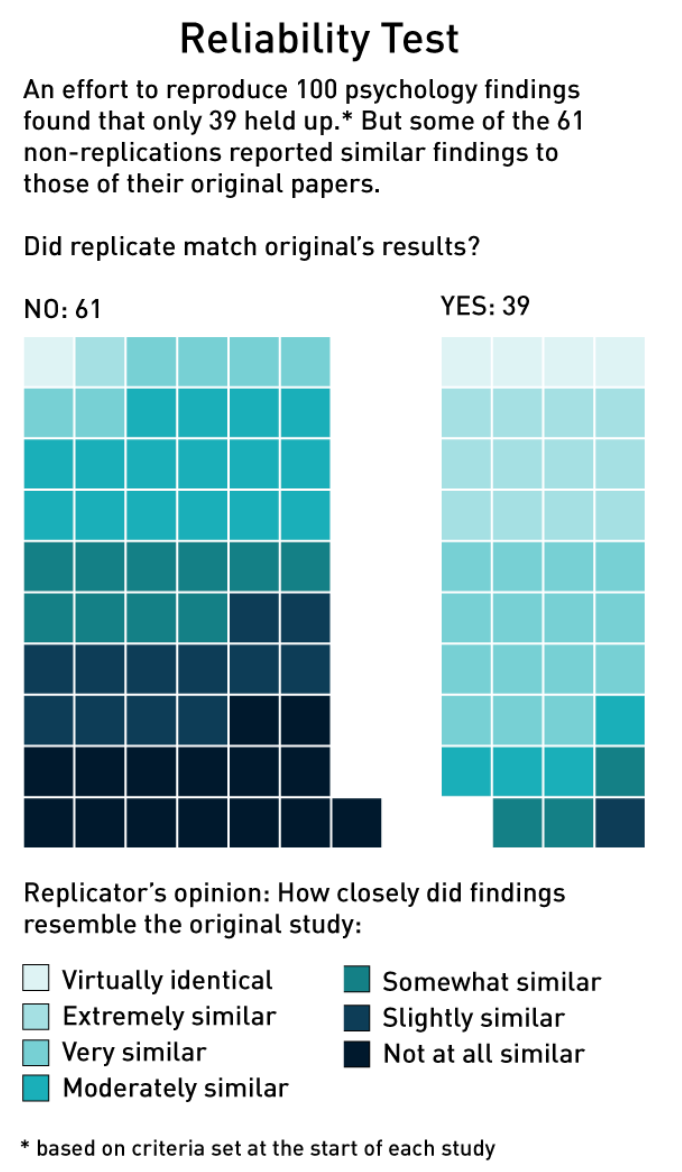
\includegraphics[width=0.8\textwidth]{figures/reliability_test.png}
  \end{columns}
    
\end{frame}


\begin{frame}
  \frametitle{Replication in Psychology (cont.)}

  Some more suprising results from the replication project:
  \begin{itemize}
    \item 97\% of original studies had significant results (p < 0.05)
    \begin{itemize}
        \item But only 36\% of replications had significant results
    \end{itemize}
    \item 47\% of original effect sizes were in the 95\% confidence interval of the replication effect size
    \item Replication effects (Mr = .197, SD = .257) were half the magnitude of original effects (Mr = .403, SD = .188)
  \end{itemize}
\end{frame}


\begin{frame}
  \frametitle{The Decline Effect}
  
  \begin{block}{The Decline Effect}
      Idea that effect sizes tend to decrease with replication
  \end{block}
  
  \begin{columns}
    \column{0.5\linewidth}
    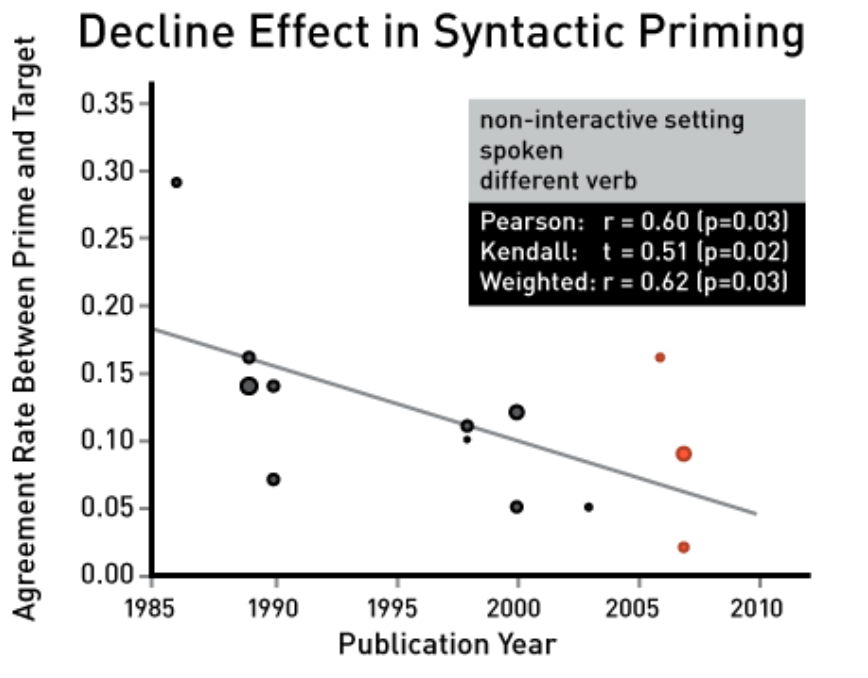
\includegraphics[width=0.95\linewidth]{figures/decline_effect.png}
   
    \column{0.5\linewidth}
    Richard Kunert looked at articles about syntactic priming
    \begin{itemize}
      \item This was a theory pioneered by Kathryn Bock in an 1986 arcicle in the journal \textit{Cognitive Psychology}
      \item The idea is that language users choosing between sentence structures will unconciously adopt a structure that they just heard
    \end{itemize}
  \end{columns}

\end{frame}

\begin{frame}
  \frametitle{The Decline Effect}

  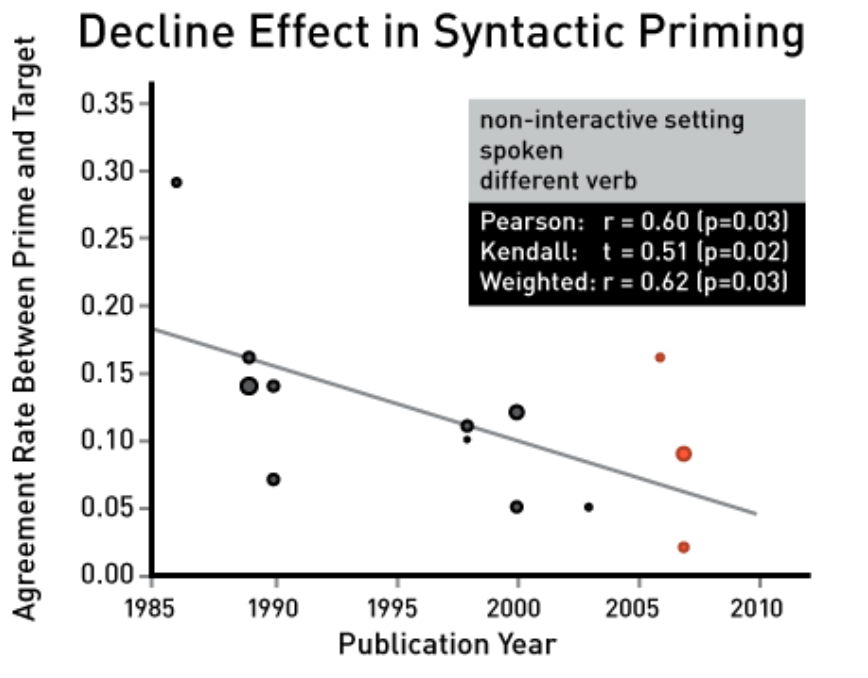
\includegraphics[width=0.95\linewidth]{figures/decline_effect.png}
\end{frame}


\begin{frame}
  \frametitle{Suspicions of Science}
  
  \textbf{Replication efforts, along with some high-profile discredited results, have led to a culture that's suspicious of science as a whole}
  
  \begin{center}
    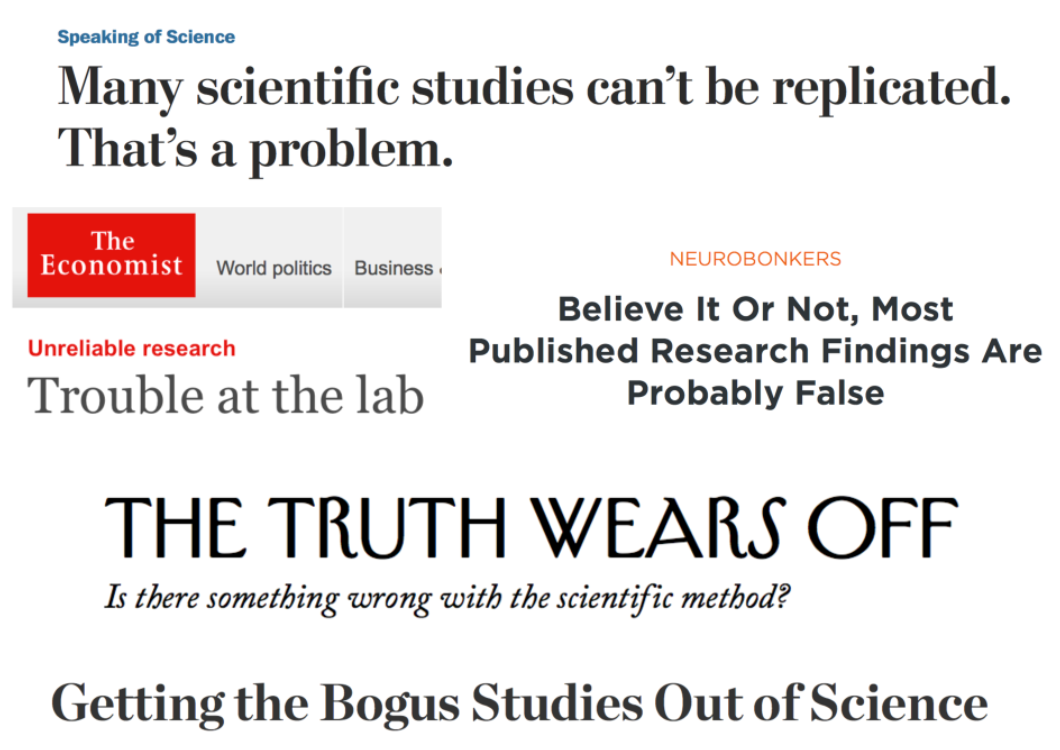
\includegraphics[width=.8\textwidth]{figures/news_headlines.png}
  \end{center}
    
\end{frame}


\begin{frame}
  \frametitle{What is the problem?}
  
  \textbf{Is this a problem with health science and psychology?}
  \begin{itemize}
      \item Unfortunately, most other fields just haven't undertaken large-scale reproduction efforts
      \item Eg. Brooks et al. write in \textit{Empirical Foundations of Computer Science} about the pressing need to replicate experimental computer science studies
  \end{itemize}
  
  \textbf{Is this just a problem with academic journals?}
  \begin{itemize}
      \item Hopefully, the examples of cancer research and software development show that companies rely on academic studies to develop products
      \item As we'll see, the underlying factors that lead to a crisis of reproducibility aren't unique to academic journals
      \item If anything, academic journals still set a good example for research; problems may be even worse in industry
  \end{itemize}
    
\end{frame}


\begin{frame}
  \frametitle{Conclusion}

This week, we're going to explore the factors that contribute to the reproducibility crisis

  \begin{itemize}
    \item First, we'll look at factors within an individual study that may inflate the Type I error rate
    \item Second, we'll look at the issues that affect entire research fields when multiple teams work on similar projects
  \end{itemize}
  
  \textbf{Ultimate goal:} Understand intricacies of the scientific method and become a more responsible consumer and practitioner of research
\end{frame}



\subsection{Single Studies and Inflated Error Rates}

\begin{frame}
  \frametitle{Reproducibility for a Single Study}
  
  \begin{itemize}
    \item We want our Type I error rate to be a manageable 0.05
    \item But some high-profile examples five the impression that actual error rates may be much higher than this
  \end{itemize}
    
\end{frame}

\begin{frame}
  \frametitle{Example: Feeling the Future}
  Daryl Bem, "Feeling the Future: Experimental Evidence for Anomalous Retroactive Influences on Cognition and Affect" \textit{Journal of Personality and Social Psychology (JPSP).}
  \begin{itemize}
    \item Nine separate experiments conducted to see if individuals could predict future events
    \item Over 1,000 subjects
  \end{itemize}
\end{frame}

\begin{frame}
  \frametitle{Feeling the Future}

  \begin{block}{Experiment Instructions}
    \footnotesize{"This is an experiment that tests for ESP. It takes about 20 minutes and is run completely by computer.

      First you will answer a couple of brief questions. Then, on each trial of the experiment, pictures of two curtains will appear on the screen side by side. One of them has a picture behind it; the other has a blank wall behind it.

      Your task is to click on the curtain that you feel has the picture behind it. The curtain will then open, permitting you to see if you selected the correct curtain. There will be 36 trials in all. Several of the pictures contain explicit erotic images (e.g., couples engaged in nonviolent but explicit consensual sexual acts).

      If you object to seeing such images, you should not participate in this experiment."}
  \end{block}
\end{frame}


\begin{frame}
  \frametitle{Feeling the Future: Results}

  Under the null hypothesis that subjects could not predict the future, we would expect them to select the right door 50\% of the time  
  \begin{itemize}
    \item \textbf{For erotic pictures, subjects were right 53.1\% of the time}, which was statistically significant
    \item \textbf{For non-erotic pictures, they were right 49.8\% of the time} (non-significant)
    \item In fact, Bem reported statistically significant results for eight of his nine experiments 
    \item They all showed slight but significant evidence for ESP
    \item Bem's paper caused a great deal of debate among psychologists
    \begin{itemize}
      \item Bem was a respected researcher
      \item The \textit{Journal of Personality and Social Psychology} is an upper-tier journal
    \end{itemize}
  \end{itemize}
    
\end{frame}


\begin{frame}
  \frametitle{Feeling the Future: Replication}
  
  \begin{itemize}
    \item Other researchers immediately started replicating Bem's studies
    \item These replications all failed to find evidence for ESP
    \item Many people wanted to know what went wrong and whether other studies could be trusted.
    \item You might wonder if Bem fabricated his data, but most observers don't believe so.
    \item Most likely, he really believed his findings

  \end{itemize}
    
\end{frame}


\begin{frame}
  \frametitle{Understanding \textit{p}-values}
  
  \begin{itemize}
    \item How is it possible that Bem got so many significant p-values?
    \item Shouldn't a p-value only be significant 5\% of the time, if the null is true?
    \begin{itemize}
        \item You may wonder if p-values can't be trusted
    \end{itemize}
    \item Bem's study gives us a good case study to help us understand exactly how the frequentist framework works.
  \end{itemize}
  
  \begin{block}{\textit{p}-values still do work, but they are often misapplied and misinterpreted}
    The $p$-value you get from statistical software is valid only under very strict conditions: You collect one dataset, never look at it, then you conduct one statistical test in isolation.
    \begin{itemize}
      \item Then your Type I error rate will be 5\%.
    \end{itemize}
  \end{block}


    
\end{frame}


\begin{frame}
  \frametitle{Understanding \textit{p}-values (cont.)}
  
  \begin{block}{When you don't meet these conditions, you may still be able to use a p-value, but you will have to correct it in some way}
    Statisticians use \textit{p-}value corrections to make sure that the Type I error rate stays at .05
  \end{block}
  
  \begin{itemize}
    \item  It turns out that the \textit{p-} values for a test (and statistical significance) can depend on some surprising things:
    \begin{itemize}
      \item What other tests you run
      \item When you come up with your theory
      \item What you would have done if you had gotten different data
    \end{itemize}
    \item We'll talk about common corrections that frequentist statisticians use
    \begin{itemize}
      \item And in doing this, we'll also shed light on how a study like Bem's could generate so many significant \textit{p-} values
    \end{itemize}
  \end{itemize}
\end{frame}



\section{Multiple Comparisons}

\begin{frame}
  \frametitle{The Multiple Comparison Problem}

  \textbf{The key to the frequentist framework is controlling error rates}
  
  \vspace{0.25in}
  
  \begin{itemize}
    \item Anything that affects your error rates affects the decisions you can draw
    \item The more opportunities you have to make an error, the higher the error rate will be 
    \item \textbf{Example:} If you perform several \textit{t}-tests, the overall probability of an error is increased
  \end{itemize}
\end{frame}


\begin{frame}
  \frametitle{Example: Green Jelly Beans}

  \begin{center}
  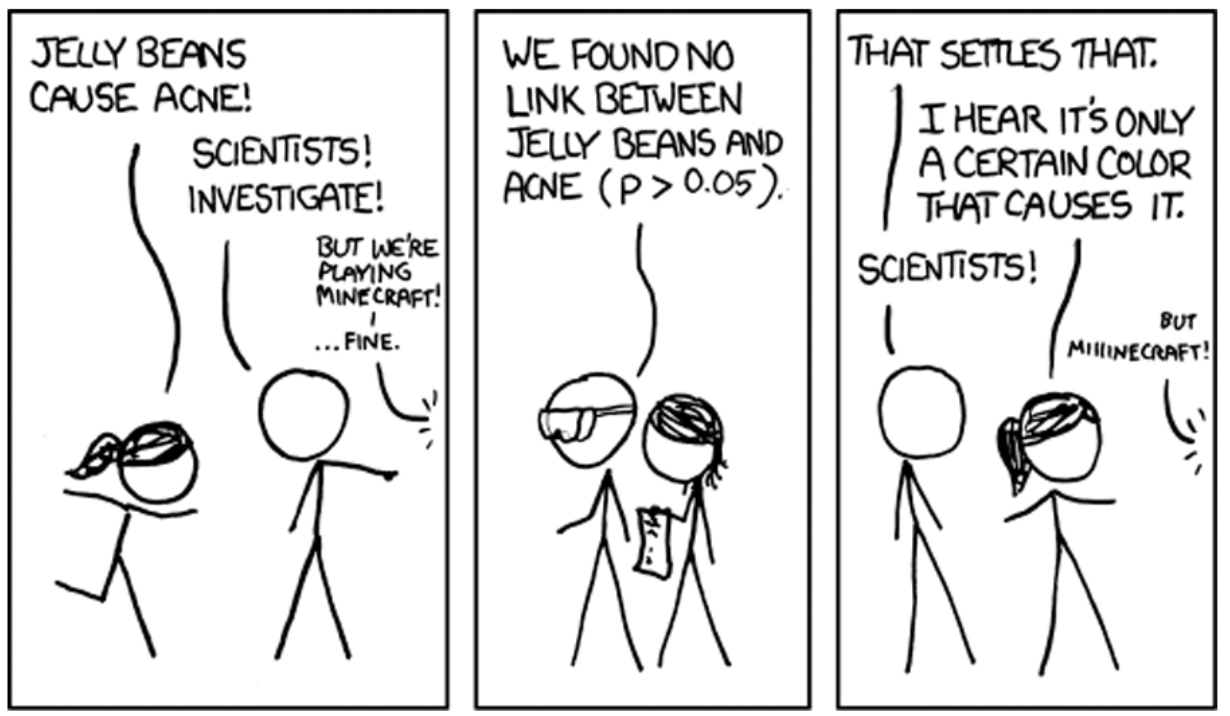
\includegraphics[width=0.9\linewidth]{figures/jelly_beans_1.png}  
  \end{center}

\end{frame}


\begin{frame}
  \frametitle{Example: Green Jelly Beans}

  \begin{center}
  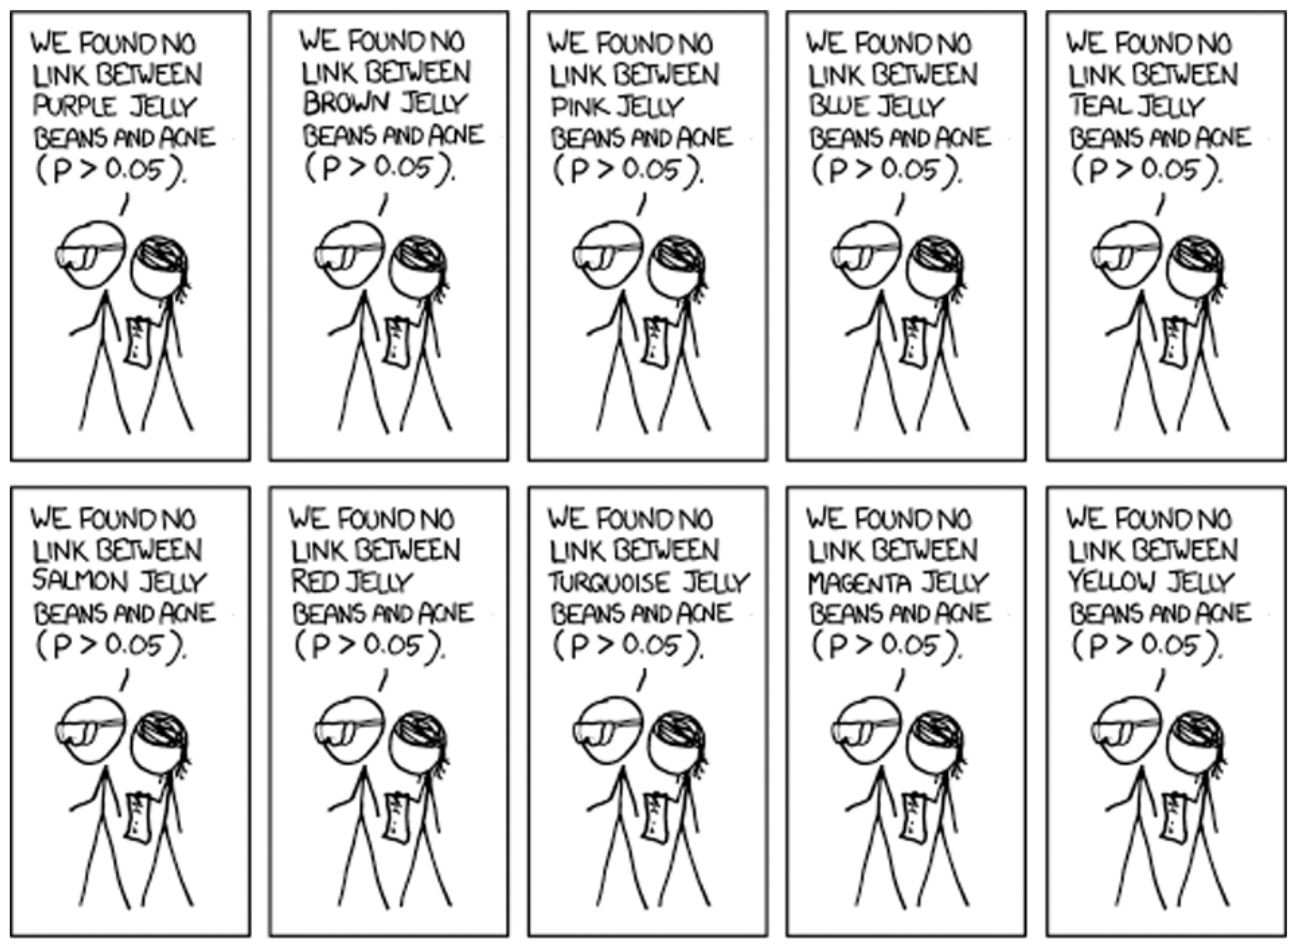
\includegraphics[width=0.9\linewidth]{figures/jelly_beans_2.png}  
  \end{center}

\end{frame}


\begin{frame}
  \frametitle{Example: Green Jelly Beans}

  \begin{center}
  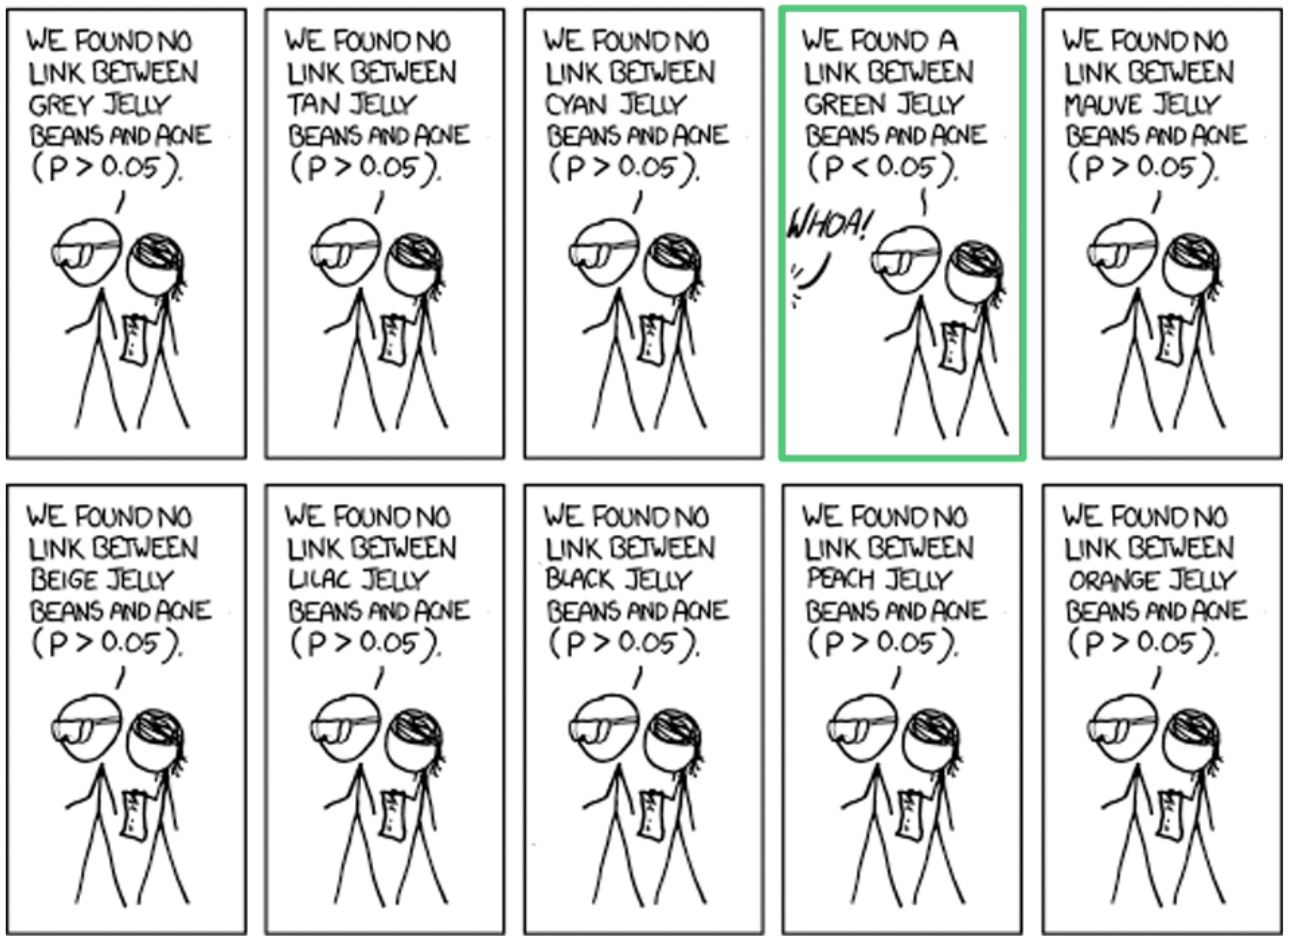
\includegraphics[width=0.9\linewidth]{figures/jelly_beans_3.png}  
  \end{center}

\end{frame}


\begin{frame}
  \frametitle{Example: Green Jelly Beans}

  \begin{center}
  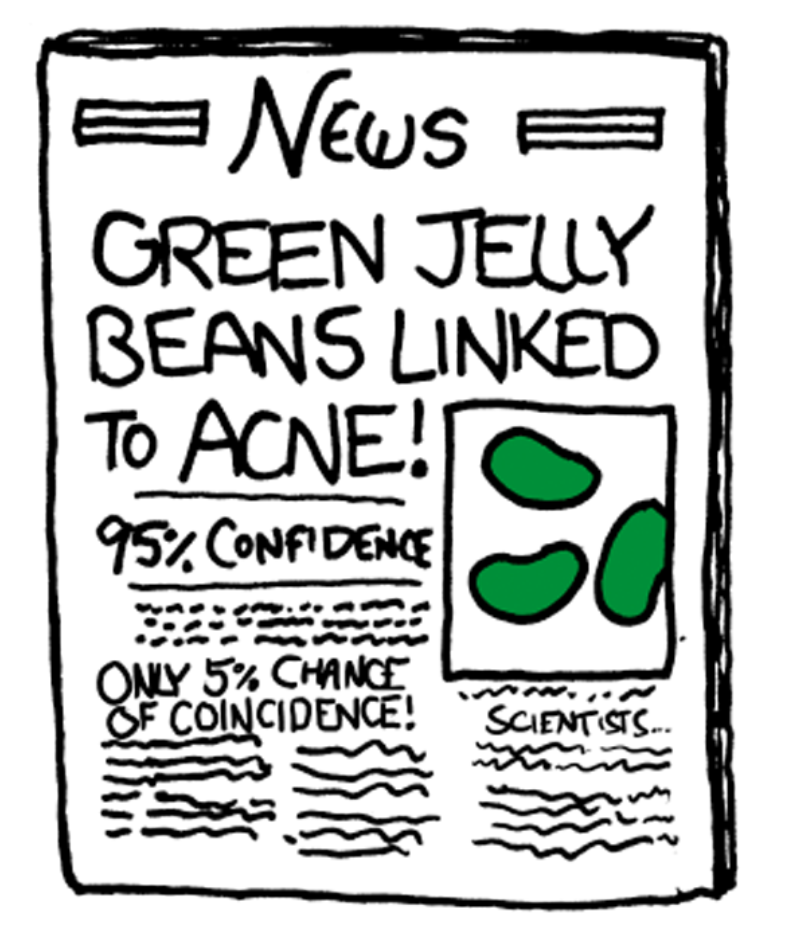
\includegraphics[width=0.6\linewidth]{figures/jelly_beans_4.png}  
  \end{center}

\end{frame}


\begin{frame}
  \frametitle{Family-Wise Error Rate}

  \begin{block}{Family-wise error rate}
    The probability, assuming all null hypotheses are true, of getting at least one Type I error
  \end{block}
  
  One possible response: running a correction on your \textit{p}-values, so the family-wise error rate returns to 0.05
\end{frame}

\begin{frame}
  \frametitle{Family-Wise Error Rate}
    
  \begin{block}{Bonferroni Correction}
    \begin{itemize}
      \item Simplest method
      \begin{itemize}
        \item If you perform $n$ comparisons, multiply each \textit{p}-value by $n$, then compare to the normal value of 0.05
        \item Equivalently, leave the \textit{p}-values the same, but check them against a threshold of $\frac{0.05}{n}$
      \end{itemize}
      \item Considered conservative
      \begin{itemize}
        \item Type I error rate may be quite a bit lower than 0.05
        \item The odds of a type 2 error are increased
        \item It may become difficult to have a significant result with a large number of comparisons
      \end{itemize}
    \end{itemize}
  \end{block}
  
\end{frame}


\begin{frame}
  \frametitle{Family-Wise Error Rate}

  \begin{block}{Interpretation of Test}
    Depends on what other tests you run
  \end{block}
  
  \begin{itemize}
      \item Critics of Neyman-Pearson approach complain that this does not make sense
      \begin{itemize}
        \item Shouldn't the evidence from a test only depend on the results of that test?
        \item Shouldn't the green jelly bean data be all that matter when studying green jelly beans?
      \end{itemize}
      \item We should have much less trust in Researcher A's conclusions since she was testing everything in sight
      \item We instinctively know that other tests matter because it could have easily been another color that was significant
  \end{itemize}
  
\end{frame}


\begin{frame}
  \frametitle{What is a family?}
    
  \textbf{This question is driven by theory}
  
  \begin{itemize}
    \item \textbf{Example:} The spectral dermatologist is not surprised that green jelly beans cause acne
    \begin{itemize}
      \item If you believe this, you probably don't feel like the other experiments have any bearing on the evidence gathered for green jelly beans
      \item You would argue that your \textit{\p-}value should not be adjusted
    \end{itemize}
    \item You have to decide whether to define your family of tests in terms of the theory
    \begin{itemize}
      \item One factor to consider is when you came up with the theory
    \end{itemize}
  \end{itemize}
\end{frame}


\begin{frame}
  \frametitle{Planned vs. Post Hoc Comparisons}

  \textbf{Timing of a Theory can make a difference in interpreting frequentist results}

  \vspace{0.2in}
  
  \begin{columns}[t]
  \column{0.35\linewidth}
    \textbf{Post hoc}
    \begin{itemize}
      \item Making comparisons and coming up with compelling theory to support link between variables \textbf{\textit{after} seeing data}
      \item Correction recommended for making comparisons
    \end{itemize}
    
  \column{0.65\linewidth}
  \textbf{Planned}
  \begin{itemize}
    \item Announcing well-motivated theory before running study
    \item Probably more convincing
    \item Easy to do in regression framework
    \item Could represent green jelly beans with dummy variable
    \item Can incorporate other planned comparisons that you are interested in
    \item No correction recommended (eg. not usually applied for estimating multiple coefficients in a linear regression)
  \end{itemize}
  
  \end{columns}

\end{frame}


\begin{frame}
  \frametitle{Other Considerations}
  
  \textbf{If you have other data that you don't want to throw away:}
  \begin{itemize}
    \item Run the planned comparison for the theory at the nominal level
    \item Separately run the post hoc tests wit ha correction
  \end{itemize}
 
 \vspace{0.2in}
 
  \textbf{If you put several tests in your research paper but they seem to be testing totally different theories (eg. green jelly beans and classical ballet):}
  \begin{itemize}
    \item You test each but believe the mechanisms that link each to the outcome variable are unrelated
    \item You still run an inflated risk of reporting at least one Type I error
    \item Present each to the reader as separate experiments to avoid a correction that may be overly conservative
  \end{itemize}
    
\end{frame}


\begin{frame}
  \frametitle{Deciding When to Correct}
  
  \begin{block}{Deciding When to Correct is Partly Cultural}
    Different fields of research employ very different standards
  \end{block}

  \textbf{Clinical studies tend to use corrections quite a bit}
  \begin{itemize}
    \item Mistakes can be costly in fields like medicine
    \item A disciplined approach is recommended by Moye (2008):
    \begin{itemize}
      \item Correct all primary endpoints of a study to bring Type I error rate to 0.05 (confirmatory)
      \item Do not correct secondary endpoints (supportive)
    \end{itemize}
  \end{itemize}
  
  \vspace{0.2in} 
  
  \textbf{The field of economics rarely uses corrections}
  \begin{itemize}
    \item Transparency is emphasized
    \item Theory should be presented clearly
    \item All tests conducted should be reported
  \end{itemize}
  
\end{frame}


\begin{frame}
  \frametitle{Takeaways}
  
  \begin{enumerate}
    \item The question of when to correct is contextual and often difficult to answer
    \item It is important to look beyond \textit{p-} values
    \begin{itemize}
        \item Did the researchers go looking for a specific effect, or are they fishing?
        \item What other results, including those from other studies, could be understood to fall in the same family?
        \item Has the hypothesis been supported by multiple studies?
    \end{itemize}
    \item Decide how convincing the results are and whether you would run a correction yourself
  \end{enumerate}
    
\end{frame}


\section{Stopping Rules}

\begin{frame}
  \frametitle{A Common Scenario}

  \begin{itemize}
    \item Research A gathers 30 subjects to see if his drug reverses hair loss
    \item He compares the treatment and control group and his \textit{t-}test is not quite significant at the .05 level
    \begin{itemize}
      \item Say \textit{p} = .06
      \item The difference is in the right direction
    \end{itemize}
    \item Researcher A realizes how close he is and gathers 10 more subjects for his study
    \begin{itemize}
      \item Now he has a total of 40 subjects to test
      \item Maybe a nominal \textit{t}-test comes out significant, \textit{p} = .04
    \end{itemize}
  \end{itemize}
\end{frame}

\begin{frame}
  \frametitle{A common Scenario (cont.)}
  
  \textbf{Does this result convince you that the drug works?}
  \begin{itemize}
      \item What's the Type I error rate?
      \item Assuming the drug has no effect, there's already a 5\% chance of a Type I error after 30 subjects
      \begin{itemize}
          \item Testing again after 40 subjects can only increase the risk of a Type I error
      \end{itemize}
      \item Research A \textit{cannot} test his 40 subjects without a correction
      \begin{itemize}
          \item Since he already accrued a 5\% chance of error, he cannot reject the null, no matter how many more subjects he gathers!
      \end{itemize}
  \end{itemize}
  
   \textbf{A better strategy: correct both \textit{p}-values, at 30 subjects as well as 40 subjects, so that the total Type I error rate is 5\%}
\end{frame}


\begin{frame}
   \frametitle{Another example study}

   Suppose Researcher B gathers all 40 subjects at once and gets the exact same data A (\textit{p} = .04)   
   \begin{itemize}
       \item Researcher B does not need a correction and can reject the null hypothesis
       \item Researcher A has the same data as Researcher B, and A did not actually stop gathering data after 30 subjects
   \end{itemize}
   
   \textbf{The fact that Researcher A would have stopped if his first \textit{t}-test was significant changes our interpretation of results}
   \begin{itemize}
       \item A critic of the Neyman-Pearson approach might say that this doesn't make sense -- our interpretation of the data depends on events that didn't actually happen
       \begin{itemize}
           \item Shouldn't the same data always lead to the same conclusion?
           \item But shouldn't the fact that research A has more chances to get a significant result make you doubt his results?
       \end{itemize}
   \end{itemize}
    
\end{frame}


\begin{frame}
   \frametitle{A Determined Researcher}
   
   Suppose that Research A kept going:
   \begin{itemize}
       \item He recruits 30 subjects and computes a \textit{t}-test at nominal level
       \item If the \textit{t}-test is non-significant, he collects 10 more subjects and runs a \textit{t}-test on the whole group
       \item If his last \textit{t}-test is non-significant, he keeps repeating 
   \end{itemize}
   
   \begin{exampleblock}{Researcher A announces that he got a significant result}
   \begin{itemize}
       \item How convinced should you be that the drug works?
       \item What's the Type I error rate?
   \end{itemize}
   \end{exampleblock}

   \begin{itemize}
       \item Researcher A is guaranteed to get a significant \textit{t}-test eventually
       \begin{itemize}
           \item It's a basic mathematical property of infinite sequences
       \end{itemize}
       \item This procedure has an alpha of 1:you always knew Research A was going to come and claim significance, so there's no information in this fact
   \end{itemize}
\end{frame}


\begin{frame}
    \frametitle{Another Explanation}
   
    \textbf{Remember that we're computing the probability of our data (or more extreme data), given our null hypothesis}
    \begin{itemize}
       \item This is an objective probability, depending on the collective rather than the single experiment
       \item We imagine an infinite sequence of hypothetical experiments conducted assuming the null hypothesis
    \end{itemize}
    
    \vspace{0.25in}
    
    \textbf{Each experiment is conducted according to the stopping rules the experimenter uses}
    \begin{itemize}
        \item Researcher A: some  experiments end after 30 subjects, some after 40, and so forth
        \item Researcher B: all experiments end after 40 subjects
    \end{itemize}


\end{frame}

\begin{frame}
    \frametitle{Another Explanation (cont.)}

    \textbf{Events that don't happen are important because we have to see how likely our results were compared to all the other results that are possible}
    \begin{itemize}
       \item This tells us how significant the data is
       \item Events that don't occur can affect what your data is telling you
       \item Clever critics poke fun at this paradoxical result
   \end{itemize}
\end{frame}

\begin{frame}
   \frametitle{\textit{p-}Values and Kung Fu}
   
   \begin{center}
       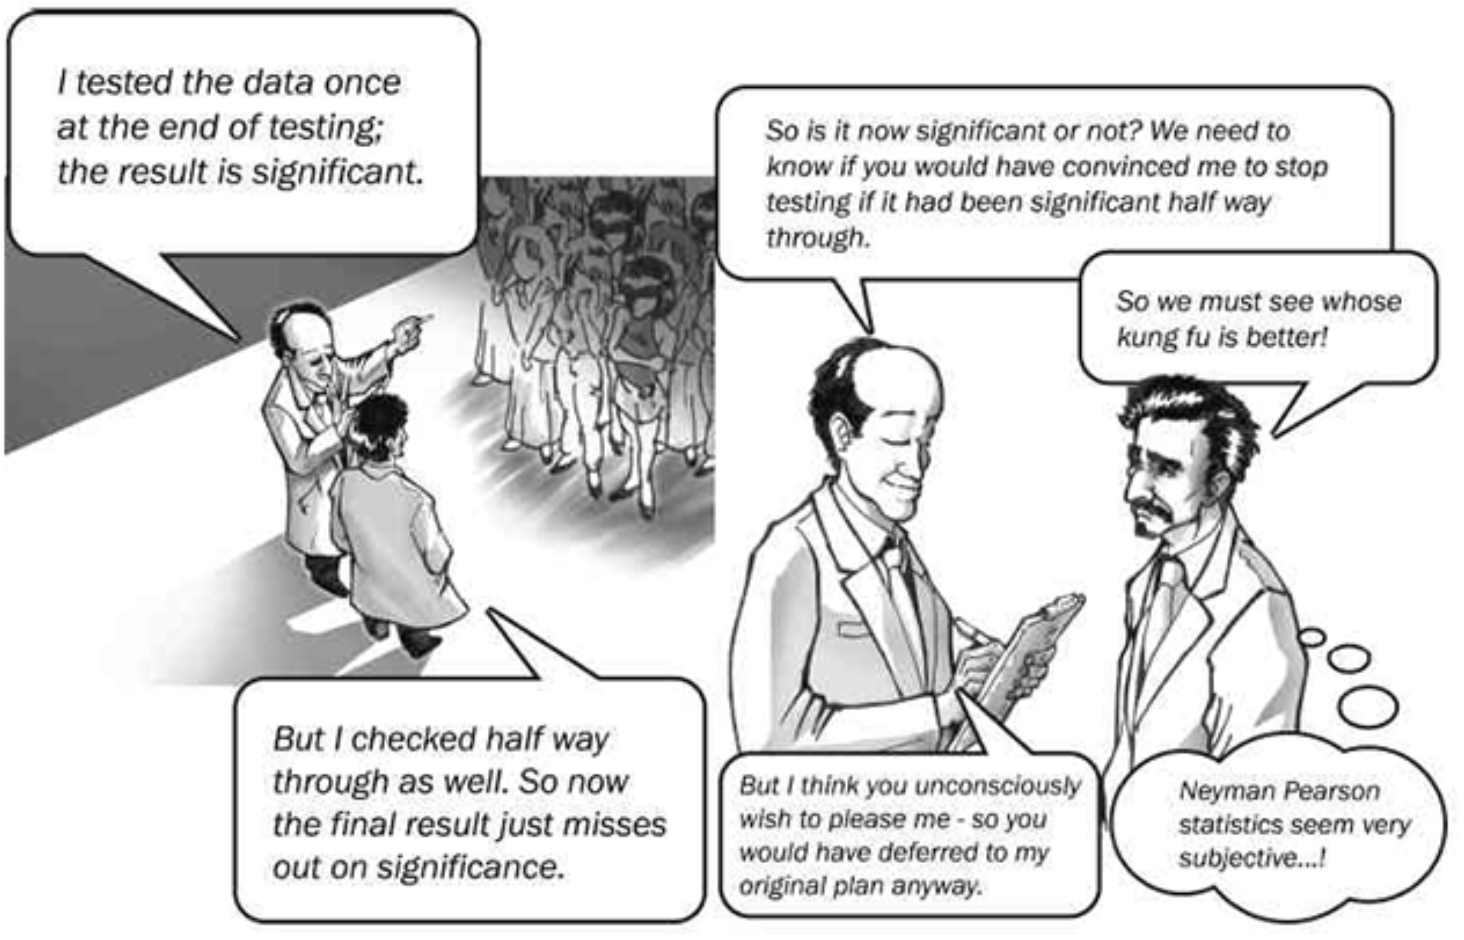
\includegraphics[width=1.0\linewidth]{figures/kung_fu_cartoon.png}
   \end{center}
    
\end{frame}


%Consider cutting this example at course iteration
\begin{frame}
   \frametitle{\textit{p-}Values and Kung Fu}
   
   In this comic taken from Dienes, two scientists realize after the fact that they have different stopping rules
   \begin{itemize}
       \item The final \textit{p-}value will have to be corrected if the experiment would have stopped halfway through if the second scientist's test was significant
       \begin{itemize}
           \item But would it have stopped?
           \item It seems the scientists didn't agree to this in advance
       \end{itemize}
       \item They try to figure out whether the experiment would have stopped
       \item The result depends on who would convince the other whose kung fu is better!
       \item Maybe the kung fu outcome will depend on the researchers' desires to please each other
       \begin{itemize}
           \item Those desires are unconscious, so how can we compare them?
       \end{itemize}
   \end{itemize}
    
\end{frame}

\begin{frame}
    \frametitle{Takeaways}
    
    \begin{enumerate}
        \item The sensitivity of frequentist statistics to events that don't occur is controversial
        \item Many critics, Bayesian statisticians in particular, think that the same data should always lead to the same conclusion
        \item You can decide if this is a strength or weakness of the approach, but know the intuition behind why events that don't occur may change your understanding of the data
    \end{enumerate}
\end{frame}


\section{In Defense of Frequentists}

\begin{frame}
    \frametitle{In Defense of Frequentists}
    
    \textbf{There are certainly many quriks to the Neyman Pearson approach}
    \begin{itemize}
        \item It has many critics
        \item What we conclude from a test may depend on several things
        \item This is unsettling to many people
    \end{itemize}
    
    \textbf{But take a moment to think of how clever all this is}
    \begin{itemize}
        \item We want a system for learning truths about the world, knowing that we may not agree on how likely hypotheses are
        \item We may not even be able to imagine what alternate hypotheses are out there!
    \end{itemize}
    
\end{frame}


\begin{frame}
    \frametitle{In Defence of Frequentists (cont.)}
    
    \textbf{But take a moment to think of how clever all this is}
    
    \begin{itemize}
        \item We define probability in terms of long-run frequencies
        \item Even though we can't discuss the probability that our null is true, we know the probability of accidentally rejecting it if it is true
        \begin{itemize}
            \item We've managed to define our error rate in terms of long-run frequencies
        \end{itemize}
        \item We have a system that makes very minimal assumptions about the world, just looking at one hypothesis in isolation
        \item The \textit{p-} value is a measure of how consistent the hypothesis is with the data
        \begin{itemize}
            \item \textit{p-} values depend on researcher intentions, stopping rules, etc
            \item These are all responses to things that inflate our error rate
            \item There will always be Type I errors
            \item Science progresses when we come up with hypotheses that survive repeated testing
        \end{itemize}
    \end{itemize}
    
\end{frame}


\section{Researcher Degrees of Freedom}
\subsection{So many places to bury those skeletons}

\begin{frame}
    \frametitle{Back to ESP}

    \textbf{Now that we have seen some of the complexity that comes with correctly applying the frequentist framework, what does that tell us about Bem's ESP study?}   
    \begin{itemize}
        \item We can't always interpret a nonimal \textit{p-}value we get from statistical software directly
        \item The statistical significance of our data depends on factors like:
        \begin{enumerate}

            \item Any other tests we've conducted on the same data
            \item When we came up with our theory
            \item What our rules are for when we stop collecting data
        \end{enumerate}
        \item We can find elements similar to all three of these in Bem's procedure
    \end{itemize}
    

\end{frame}


\begin{frame}
    \frametitle{Stopping Rules}
    
    \textbf{Bem himself said that he peeked at the data as it was coming in}
    \begin{itemize}
        \item Wagenmakers et al. noticed that the number of subjects in each experiment was negatively related to the effect size
        \item This is a pattern we expect to see when a research uses an optional stopping rule
    \end{itemize}
    
    \begin{block}{Bad Science: An Optional Stopping Rule}
      Collecting more participants as long as a test is non-significant
    \end{block}
    
    \textbf{Since Bem used an optional stopping rule, we know that his \textit{p-}values cannot be interpreted at a nominal level}
    \begin{itemize}
        \item We would need some sort of correction
        \item It might be impossible to design one without knowing exactly how Bem determined when to stop each experiment
    \end{itemize}
\end{frame}


\begin{frame}
    \frametitle{Multiple Comparisons}
    
    \begin{block}{From Bem's Experiment \#6:}
        \textit{The hit rate on control trials was at chance for exposure frequencies of 4, 6, and 8. On sessions with 10 exposures, however, it fell to 46.8\%, t(39) = -2.12, two-tailed \textit{p} = .04}
    \end{block}

    \textbf{Here, we clearly have four comparisons}
    \begin{itemize}
        \item One turned out slightly significant at the nominal level
        \item We know that these \textit{p-}values require a correction
    \end{itemize}
    
    \textbf{At other times, we're led to suspect that Bem performed comparisons other than the ones he published}
    \begin{itemize}
        \item Consider that Bem's Experiment \#1 tested not just erotic pictures, but also:
        \begin{itemize}
            \item Neutral pictures
            \item Negative pictures 
            \item Positive pictures
            \item Pictures that were romantic but non-erotic
        \end{itemize}
    \end{itemize}
\end{frame}

\begin{frame}
    \frametitle{Multiple Comparisons (cont.)}
    
    \textbf{Only the result for erotic pictures appears in the paper}
    \begin{itemize}
        \item Did Bem not examine the other categories?
        \item Or did he look at the data and choose the one that was most promising?
    \end{itemize}
    
    \textbf{Bem also mentions other variables that he discarded for having no effect}
    \begin{itemize}
        \item Openness to experience
        \item Belief in psi
        \item Belief that one has had some psi experiences in everyday life
    \end{itemize}
    
    \vspace{0.2in}
    
    \textbf{ \large{All in all, this amounts to a large number of comparisons}}
\end{frame}


\begin{frame}
    \frametitle{Post Hoc Comparisons}
    
    \textbf{It seems that Bem's comparisons weren't driven by a pre-existing theory}
    \begin{itemize}
        \item Instead, he seemed to come up with theory to match his results
        \item In Experiment \#5, Bem reports a significant \textit{t-}test for women, but not for men
        \item Not clear why he wanted to test for gender in the first place
        \item Bem does offer some analysis of the gender difference:
    \end{itemize}

    \begin{quote}
        "It seemed possible that the men were simply less aroused than the women by the negative pictures; male raters rated every one of the negative pictures in the set as less negative and less arousing than did female raters."
    \end{quote}
    
    \textbf{This analysis comes after the data is analyzed}
    \begin{itemize}
        \item Since the theory is applied post hoc, most statisticians would see this as a reason to recommend a correction
    \end{itemize}

\end{frame}


\begin{frame}
    \frametitle{Glancing at Data}
    
    \begin{itemize}
        \item Bem may not have performed a formal \textit{t-}test on every category
        \item Instead, Bem may have merely glanced at the data to see which variables looked most favorable to his theory
        \item But merely glancing at data is enough to inflate Type I error rates
        \begin{itemize}
            \item You don't have to perform a statistical test
        \end{itemize}
    \end{itemize}
    
    \textbf{Glancing at your data is enough to lead you to the most promising tests, implicitly discarding others}
    \begin{itemize}
        \item If you're glancing at data and using your gut, it is next to impossible for a statistician to choose an appropriate correction for your \textit{p-}values
        \item How many comparisons have you really conducted by looking at the data and looking for values that jump out at you?
    \end{itemize}
    
    \textbf{ {\large Bem made many choices along the way that could have helped create a small \textit{p-} value}}
\end{frame}


\begin{frame}
    \frametitle{Researcher Degrees of Freedom}
    
    \begin{block}{Researcher degrees of freedom}
        Consist of all the choices that a researcher makes in the course of an analysis
    \end{block}
    
    \begin{itemize}
        \item When should we stop collecting data?
        \item Which observations should be excluded?
        \item Should we take a log transform of a variable? Make it binary?
        \item Which parametric or non-parametric test should we run?
        \item What control variables should we include?
        \item Should we use robust standard errors?
    \end{itemize}
    
    \textbf{We usually can't answer these questions ahead of time}
    \begin{itemize}
        \item Hundreds of choices go into a moderately sized analysis
        \item Each degree of freedom is an opportunity to create a smaller \textit{p-}value
        \item The sum total of many researcher degrees of freedom can be dramatic
    \end{itemize}
\end{frame}

\begin{frame}
    \frametitle{Researcher Degrees of Freedom (cont.)}
    
    \textbf{Here's how Bem describes his approach to data:}
    \begin{quote}
        "Let us at least become intimately familiar with the record of their behavior: the data. Examine them from every angle. Analyze the sexes separately. Make up new composite indexes. If a datum suggests a new hypothesis, try to find further evidence for it elsewhere in the data. If you see dim traces of interesting patterns, try to reorganize the data to bring them into bolder relief. If there are participants you don't like, or trials, observers, or interviewers who gave you anomalous results, place them aside temporarily and see if any coherent patterns emerge. Go on a fishing expedition for something—anything—interesting."
    \end{quote}

        \textbf{These are a lot of degrees of freedom, so we shouldn't be at all surprised to find significant \textit{p-}values}
    \begin{itemize}
        \item You could call this \textit{p-}hacking
    \end{itemize}

\end{frame}


\begin{frame}
    \frametitle{Exploratory vs. Confirmatory Research}
    
    \textbf{This is not to say that exploring a data set is bad}
    \begin{itemize}
        \item Exploratory analysis is a critical part of research
        \item However, we must understand how to interpret statistical results in context
        \item Many researchers, especially in experimental fields, recommend distinguishing between two types of research
    \end{itemize}
    
    \begin{block}{Exploratory Research}
        Getting to know a data set, looking for patterns, generating hypotheses (creativity is good)
    \end{block}
    
    \begin{block}{Confirmatory Research}
        Testing data with a specific theory in mind. You want to make as many decisions as possible before you see your data
    \end{block}
    
\end{frame}


\begin{frame}
    \frametitle{Exploratory vs. Confirmatory Research (cont.)}
    
    \textbf{You shouldn't use the same dataset for exploratory analysis and confirmatory analysis}
    \begin{itemize}
        \item If possible, it's ideal to split your dataset and save some for confirmation
        \item These are ideals that we aspire to. It's not always possible to split your dataset
    \end{itemize}
    
    \vspace{0.25in}
    
    \textbf{If you have to combine some elements of exploration and confirmation, think how to mitigate risk of inflated error rates:}
    \begin{itemize}
        \item Have a specific research question
        \item Report multiple specifications
        \item Document the choices you make so readers can perform their own analysis
    \end{itemize}
\end{frame}



\subsection{Replication and Meta-Analysis}

\begin{frame}
    \frametitle{Replication}
    
    \begin{block}{Replication}
        Different teams performing studies to address the same question (or similar questions)
    \end{block}
    
    \begin{itemize}
        \item In a well-functioning research field, studies are replicated
        \item Replication is our last line of defense against Type I errors
        \item Bem's study is a good example
        \begin{itemize}
            \item After published, several teams immediately undertook replication attempts
            \item Virtually all of these failed to reproduce Bem's evidence for ESP
        \end{itemize}
    \end{itemize}
    
\end{frame}

\begin{frame}
    \frametitle{Example}
    
    Ritchie, Stuart J.; Wiseman, Richard; French, Christopher C.; Gilbert, Sam. (March 2012). Gilbert, Sam, ed. "Failing the Future: Three Unsuccessful Attempts to Replicate Bem's 'Retroactive Facilitation of Recall' Effect". PLoS ONE.
    
    \vspace{0.25in}
    
    From their abstract:
    \begin{quote}
        "We describe three pre-registered independent attempts to exactly replicate one of these experiments, 'retroactive facilitation of recall', which examines whether performance on a memory test can be influenced by a post-test exercise. All three replication attempts failed to produce significant effects (combined n = 150; combined p = .83, one-tailed) and thus do not support the existence of psychic ability."
    \end{quote}
    
\end{frame}

\begin{frame}
    \frametitle{Example (cont.)}
    
    \textbf{Replication isn't just a defense against poorly constructed studies}
    \begin{itemize}
        \item There will always be Type I errors
        \item Under the best circumstances, the Type I error rate will be .05
        \item Replication is what lets us eventually correct these errors
        \item It is a central component of the scientific method
    \end{itemize}

    \vspace{0.25in}
    
    Another replication team summed it up by quoting Karl Popper, a philosopher who laid down early intellectual foundations for modern research:
    
    Popper (1959–2002) defined a scientifically true effect as:
    \begin{quote}
        \textit{"That which can be regularly reproduced by anyone who carries out the appropriate experiment in the way prescribed." }
    \end{quote}

\end{frame}


\begin{frame}
    \frametitle{Obstacles to Replication}
    
    \textbf{Unfortunately, as a crucial as replication is, there are significant obstacles to conducting replications}
    \begin{itemize}
        \item Recall the replication attempt by Ritchie, French, and Wiseman
        \item Three journals rejected their paper on the grounds that it was a replication (\textit{The Journal of Personality and Social Psychology, Science Brevia, and Psychological Science)  }
        \item A fourth journal, the \textit{Britich Journal of Psychology}, refused the paper after reservations from one referee
        \begin{itemize}
            \item That referee was later confirmed to be Daryl Bem
        \end{itemize}
    \end{itemize}
    
        \textbf{Unfortunately, the difficulty these researchers had in publishing their replication attempt is not atypical}
    \begin{itemize}
        \item Makel, Plucker, and Hegarty estimated that about 1.07\% of published psychology studies are replications
    \end{itemize}
    
\end{frame}


\begin{frame}
    \frametitle{Obstacles to Replication (cont.)}

    \textbf{Brian D. Earp and Jim A. C. Everett enumerated five reasons replication attempts are uncommon in psychology:}
    \begin{enumerate}
        \item Independent, direct replications of others' findings can be time consuming for the replicating researcher
        \item Replications are likely to take energy and resources directly away from other projects that reflect one's own original thinking
        \item Replications are generally harder to publish (in large part because they are viewed as being unoriginal)
        \item Even if replications are published, they are likely to be seen as 'bricklaying' exercises, rather than as major contributions to the field
        \item Replications bring less recognition and reward, and even basic career security, to their authors.
    \end{enumerate}
    
    \textbf{There are some initiatives to encourage more replication but, unfortunately, it remains far too rare in most fields }
\end{frame}


\begin{frame}
    \frametitle{Meta-Analysis, Part One}
    
    \textbf{If we're lucky enough to work in a field in which replication occurs, how do we weigh the evidence for a hypothesis?}
    
    \textit{Eg. What if there are six replication attempts and three support the original findings?}
    
    \begin{itemize}
        \item It doesn't make sense to take a vote, since we only expect 5\% of studies to find evidence if the null is true
        \item Furthermore, what if some studies are just bigger than others? 
        \item Shouldn't they count for more?
    \end{itemize}
    
    \textbf{Instead, we can conduct a meta-analysis}
\end{frame}


\begin{frame}
    \frametitle{Meta-Analysis, Part Two}
    
    \begin{block}{Meta-analysis}
        A statistical technique for combining evidence from a group of studies
            \begin{itemize}
        \item It's important that all the studies report the same measure of effect size for the phenomenon they are trying to measure
    \end{itemize}
    \end{block}
    
    \vspace{0.25in}
    
    \textbf{The objective of a meta-analysis is to create a single pooled estimate of the effect size}
    \begin{itemize}
        \item This is essentially a weighted average of the effect sizes reported from each study
        \item The weighting usually relates to the inverse of the variance
        \item This means that studies with a larger sample size will generally count more toward a pooled estimate
    \end{itemize}
\end{frame}


\begin{frame}
    \frametitle{Meta-Analysis, Part Three}
    
    \textbf{A meta-analysis is itself a research study}\
    \begin{itemize}
        \item It has a lot of the same elements that any other study does
    \end{itemize}
    
    \textbf{Researchers must first specify the procedure for determining which studies should be included in the meta-analysis}
    \begin{itemize}
        \item These are the raw data
        \item It is critical to have a systematic method for identifying data points
        \item The criteria for which studies are excluded should be as objective as possible
    \end{itemize}
    
    \textbf{There are different statistical methods for combining effect sizes into pooled estimates}
    \begin{itemize}
        \item Researchers can use fixed effects and random effects models
        \item Those are beyond the scope of today's lecture
    \end{itemize}
\end{frame}


\begin{frame}
    \frametitle{Forest Plot}
    
    \begin{columns}
    \column{0.5\linewidth}
    \begin{itemize}
        \item The selected studies are usually shown on a forest plot
        \item Each row shows an estimated effect size, along with 95\% confidence intervals
        \item The diamond represents the pooled estimate, along with a 95\% confidence interval
    \end{itemize}
        
    \column{0.5\linewidth}
    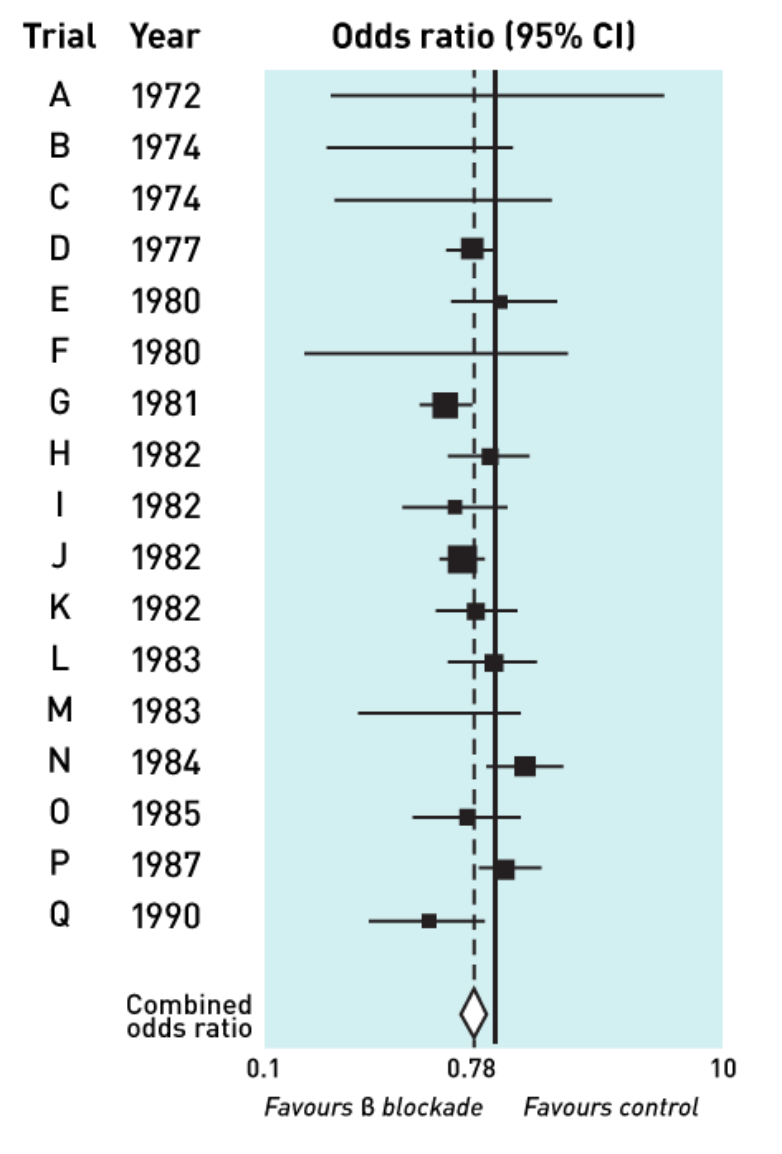
\includegraphics[width=0.9\linewidth]{figures/forest_plot.png}

    \end{columns}
    
\end{frame}

\begin{frame}
    \frametitle{Conclusion}
    
    \textbf{We've only begun to scratch the surface:} You can take an entire class about meta-analysis
    
    \vspace{0.25in}
    
    \textbf{Meta-analysis shifts our focus away from one study to groups of studies}
    \begin{itemize}
        \item This is the most important takeaway
        \item Each study is just one data point
        \item An informed reader should evaluate it in that context
    \end{itemize}
\end{frame}



\subsection{The File Drawer Problem}

\begin{frame}
    \frametitle{The File Drawer}
    
    \begin{block}{File Drawer}
        Refers to all the negative results researchers get that don't get published
    \end{block}
    
    \textbf{Bluntly, everyone likes positive results}
    \begin{itemize}
        \item Includes journal editors
        \item Positive results mean that you detected a relationship
        \begin{itemize}
            \item May support a theory
            \item Helps you write an exciting conclusion
            \item Can mean that your product works
        \end{itemize}
    \end{itemize}
    
    \textbf{Negative results just don't generate as much excitement}
    \begin{itemize}
        \item You don't accept the null, you just fail to reject it
        \item Instead of being published these negative results just sit in a file drawer and nobody finds out about them
        \item This is also called \textbf{publication bias}
    \end{itemize}
\end{frame}

\begin{frame}
    \frametitle{The File Drawer (cont.)}
    
    \textbf{Dickersin, Chan, Chalmers, Sacks, and Smith conducted a survey of 156 medical researchers}
    \begin{itemize}
        \item Out of the 1041 \textit{published} RCTs , 55\% showed a positive result
        \item Out of the 271 \textit{unpublished} RCTs, only 14\% showed a positive result
        \item Authors of unpublished RCTs were also asked why they thought their study was unpublished
        \item Results shown in Table 3:
    \end{itemize}
\end{frame}

\begin{frame}
    \frametitle{RCT Status and Reasons for Not Publishing}

    \begin{center}
        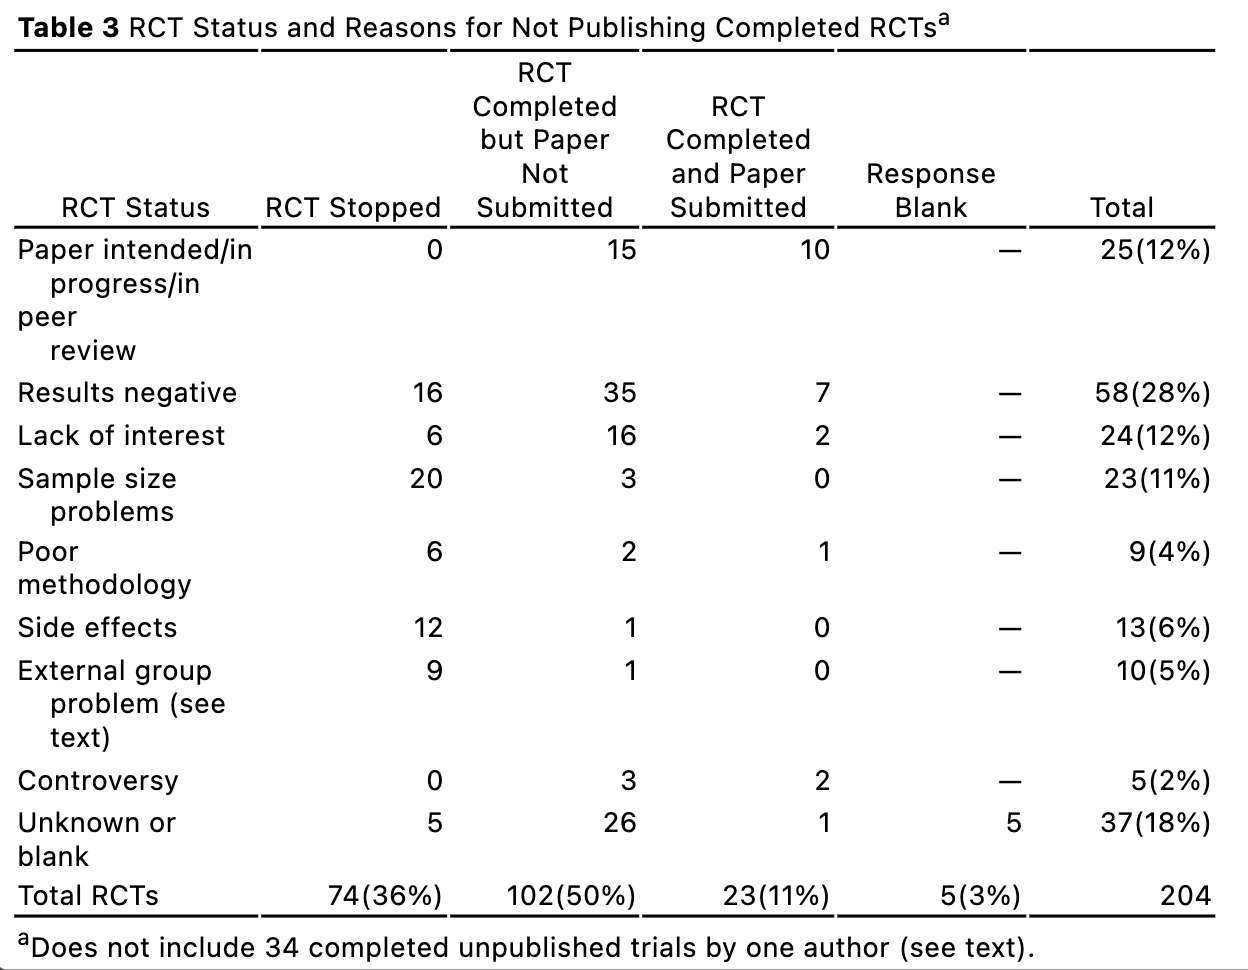
\includegraphics[width=0.9\linewidth]{figures/table_3.png}
    \end{center}
    
\end{frame}


\begin{frame}
    \frametitle{Effects of the File Drawer}
    
    \textbf{Why is the file drawer bad?}
    \begin{itemize}
        \item This is closely related to the issue of multiple comparisons
        \item Remember that your interpretation of a statistical test depends on what other tests have been conducted
        \begin{itemize}
            \item That's true in a single study, but its also true when we're talking about multiple studies
        \end{itemize}
        \item Say you read a paper that finds a statistically significant effect
        \begin{itemize}
            \item Eg. that eating kale improves reaction time
            \item What if you discover that five other research teams tested kale for reaction time and couldn't reject the null?
            \item Or maybe they tested broccoli, asparagus, lettuce, and brussels sprouts, but only the kale team found a significant results and only that team managed to publish
            \item From what you know about multiple comparisons, this context could be important for understanding the result
        \end{itemize}
    \end{itemize}

\end{frame}


\begin{frame}
    \frametitle{Detecting Publication Bias}
    
    \textbf{The file drawer effect is also a problem when we conduct a meta-analysis}
    \begin{itemize}
        \item If there's a publication bias, the studies that are published will tend to be those that find larger effect sizes
        \item As a result, our pooled estimate will be biased upward
        \item This is the GIGO principle: garbage in, garbage out
    \end{itemize}
    
    \vspace{0.25in}
    
    \textbf{If we have enough studies that measure the same effect, we may be able to detect publication bias}
    \begin{itemize}
        \item This is done with a funnel plot
    \end{itemize}
\end{frame}


\begin{frame}
    \frametitle{The Funnel Plot}
    
    \begin{center}
        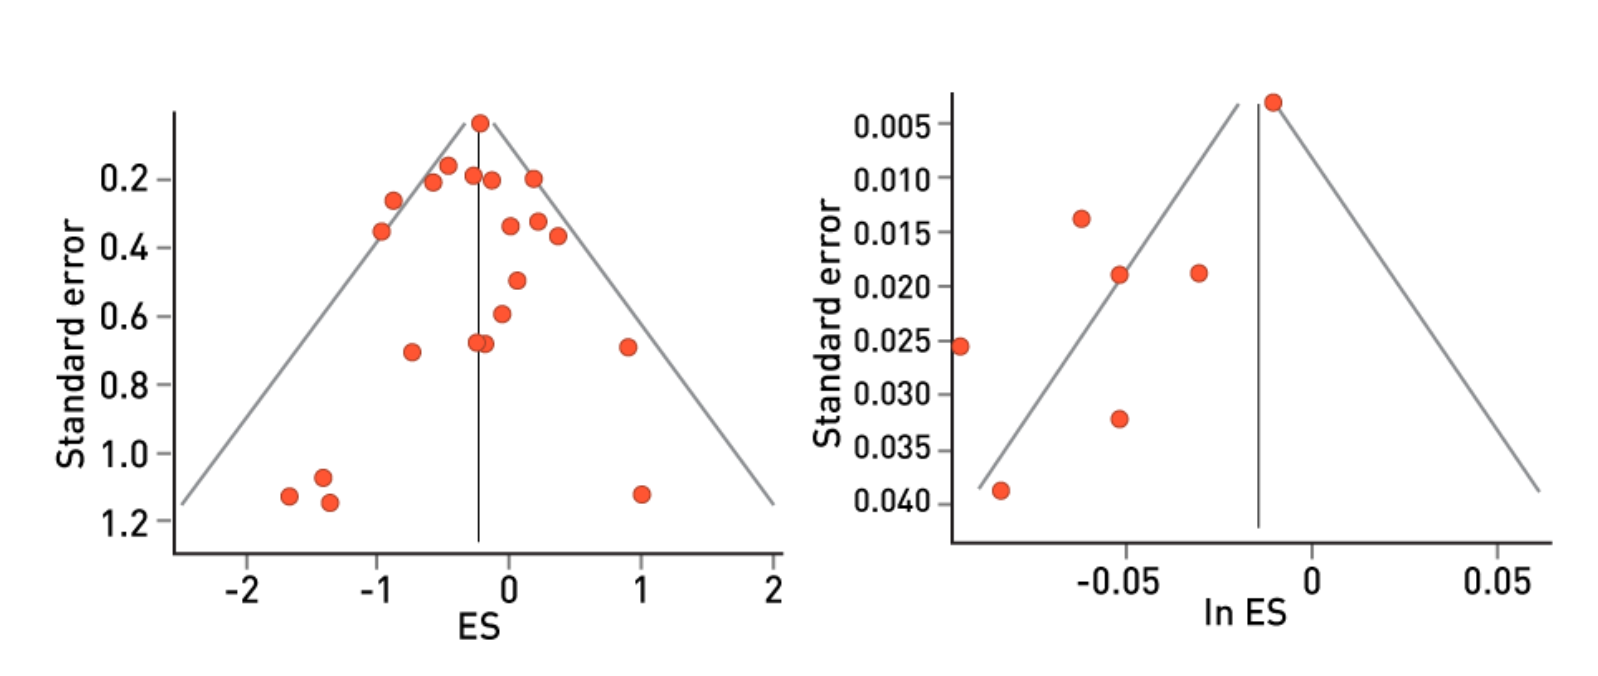
\includegraphics[width=1.0\linewidth]{figures/funnel_plot.png}
    \end{center}

\end{frame}


\begin{frame}
    \frametitle{Funnel Plot: All studies published}
    
    \begin{center}
        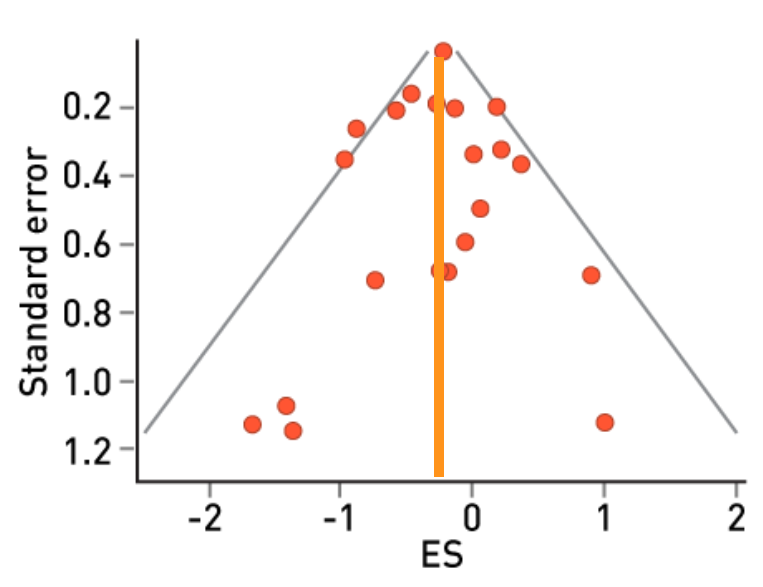
\includegraphics[width=0.75\linewidth]{figures/funnel_plot_a.png}
    \end{center}
    
\end{frame}


\begin{frame}
    \frametitle{Funnel Plot: Publication Bias}
    
    \begin{center}
        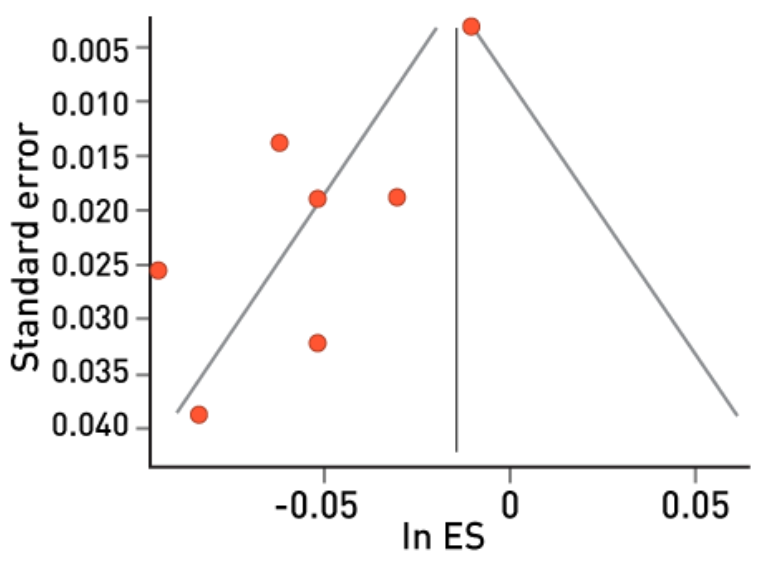
\includegraphics[width=0.75\linewidth]{figures/funnel_plot_b.png}
    \end{center}
    
\end{frame}


\begin{frame}
    \frametitle{Example: Stereotype Threats}
    
    Flore P.C., \& Wicherts J.M. (2015). Does stereotype threat influence performance of girls in stereotyped domains? A meta-analysis. \textit{J School Psychology.}
    
    \begin{itemize}
        \item Authors asked whether a stereotype threat would affect women's performance on mathematics tests
        \item Stereotype threat: a member of a stigmatized group is exposed to a negative stereotype about that group
        \item Over 100 studies were conducted on this question
        \item In a typical study, a treatment group of women might be presented with a written statement that men do better on math tests
        \item Their performance on a math test would then be measured
        \item A control group would not get the stereotype threat
        \item Four out of five meta-analyses confirmed the existence of an effect
    \end{itemize}
\end{frame}


\begin{frame}
    \frametitle{Example: Stereotype Threats (cont.)}
    
    \begin{columns}
    \column{0.5\linewidth}
        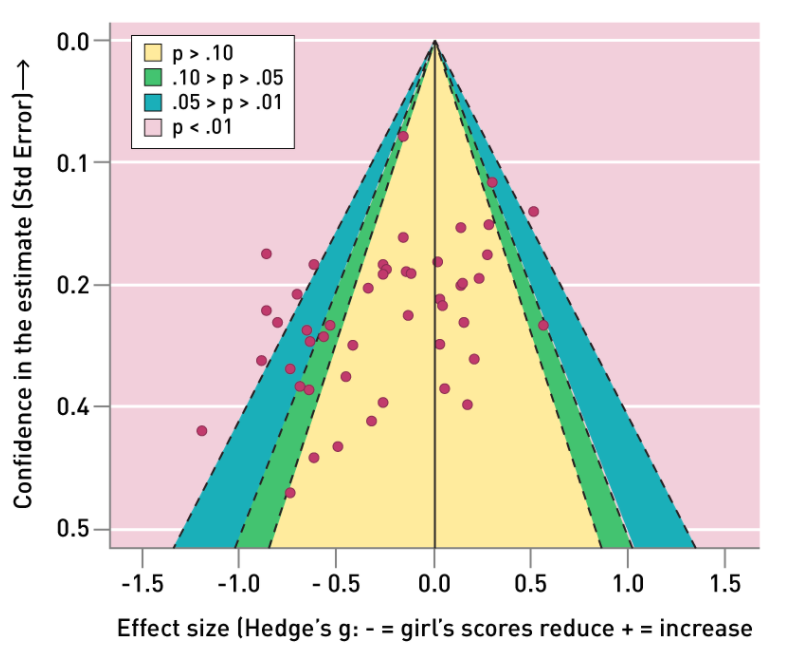
\includegraphics[width=1.0\linewidth]{figures/stereotype_threats_funnel_plot.png}
    
    \column{0.6\linewidth}
        \begin{itemize}
          \item Flore and Wicherts examined the data to evidence of a file drawer effect
          \item The funnel plot shows a distinctively non-symmetrical shape
          \item This is supported by a number of statistical tests
          \item The authors conclude that there is not evidence to establish the existence of the stereotype threat effect
          \item They advocate for a large-scale pre-registered study to address the problem
        \end{itemize}
    \end{columns}
    
\end{frame}


\begin{frame}
    \frametitle{Conclusion}
    
    \textbf{There have been some high-profile efforts to mitigate the file drawer problem}
    \begin{itemize}
        \item Some journals have a policy of accepting negative results
        \item Other repositories for negative results have sprung up
        \item Pre-registration of studies can help us by at least telling us how many studies are conducted
    \end{itemize}
    
    \textbf{The file drawer remains a major problem and something you should keep in mind when reading research}
\end{frame}



\subsection{True Relationships and False Relationships}

\begin{frame}
    \frametitle{The Positive Predictive Value}
    
    \textbf{We motivated this discussion by describing the reproducibility crisis.} 
    
    \begin{itemize}
        \item Why are so many published findings not reproducible?
        \item We spent a long time talking about Type I errors
        \begin{itemize}
            \item Why do Type I errors occur more often than we expect?
            \item Why do Type I errors persist in the literature?
        \end{itemize}
        \item The Type I error rate is important, but it's not the end of the story
    \end{itemize}
    
    \textbf{We're ultimately interested in the fraction of published results that are false, and that's not the same as the Type I error rate}
\end{frame}

\begin{frame}
    \frametitle{The Positive Predictive Value (cont.)}
    
    \textbf{Remember that Type I error rate is the probability of getting a significant result, assuming the null is true (research hypothesis is false)}
    \begin{itemize}
        \item We're interested in the probability that research hypothesis is false, given that we got a significant result: the probability inverse
        \item If the set of published significant results, some come from studies that successfully find evidence for a true research hypothesis
        \item But others are Type I errors when the hypothesis is false
        \item We call the fraction of significant findings that correspond to true relationships the \textit{positive predictive value (PPV)}
    \end{itemize}
    
    \begin{block}{Positive Predictive Value (PPV)}
        The probability, given that a research hypothesis is supported, that it is actually true
    \end{block}
\end{frame}


\begin{frame}
    \frametitle{John Ioannidis's Model, Part One}
    
    \textbf{John Ioannidis provides a simple model to explain the difference between the Type I error rate and the positive predictive value}
    \begin{itemize}
        \item Say researchers are testing a set of $c$ possible relationships
        \begin{itemize}
            \item The null hypothesis is always that there is no relationship
            \item The research hypothesis is that a relationship exists
        \end{itemize}
        \vspace{0.25in}
        \item Let $R$ be: $\frac{ \text{Number of true relationships} }{ \text{Number of false relationships} }$
        \vspace{0.25in}
        \item Let's further assume that all relationships get tested once, with
        \begin{itemize}
            \item $\alpha=$ Type I error rate
            \item $\beta=$ type 2 error rate 
        \end{itemize} 
    \end{itemize}
\end{frame}


\begin{frame}
    \frametitle{John Ioannidis's Model, Part Two}
    
    \begin{block}{Ioannidis' Model} 
    Let $t$ be the number of true relationships. Then, $c-t$ is the number of false relationships. Then, $R$, the ratio of true to false is: $R=\frac{t}{c-t}$. Multiplying and distributing,
    
    $$ 
        (R\cdot c) - (R\cdot t) = t
    $$ 
    
    Solving for $t$, the number of true relationships is, 
    
    $$
        t = \frac{(c\cdot R)}{R+1}, 
    $$
    
    and solving for $c-t$ the number of false relationships is, 
    
    $$
        \frac{c}{R+1}.
    $$
    \end{block}

\end{frame} 

\begin{frame}
    \frametitle{John Ioannidis's Model, Part Two (cont'd)}

    \begin{block}{Implications of Ioannidis's Model}
        \begin{itemize}
            \item For the $t$ true relationships, $(1-\beta)\cdot t$ are supported
            \item Number of supported true relationships: $\frac{(1-\beta)\cdot(c\cdot R)}{R+1}$
            \item For the ($c-t$) false relationships, $\alpha\cdot(c-t)$ are supported
            \item Number of supported false relationships = \large{$\frac{(\alpha \cdot c)}{R+1}$}
        \end{itemize}
    \end{block}
\end{frame}
    
\begin{frame}
    \frametitle{John Ioannidis's Model, Part Three}

    \begin{block}{Total number of significant results}
        $$
            \frac{\left[(1-\beta)\cdot R+\alpha\right]\cdot c}{R+1}
        $$
    \end{block}
    
    \begin{block}{PPV Formula}
        PPV is the number of supported true relationships divided by the total number of supported relationships, 
        $$
           \mathbf{PPV}=\frac{(1-\beta)\cdot R}{(1-\beta)\cdot R + \alpha}
        $$
        
    \end{block}

    \begin{itemize}
        \item Large $R$ (most true) + small $\beta$ (high power) $\rightarrow$ high PPV
        \item Small $R$ (most false) + large $\beta$ (low power) $\rightarrow$ small PPV
    \end{itemize}
\end{frame}    


\begin{frame}
    \frametitle{Unlikely Results}
    
    \begin{center}
        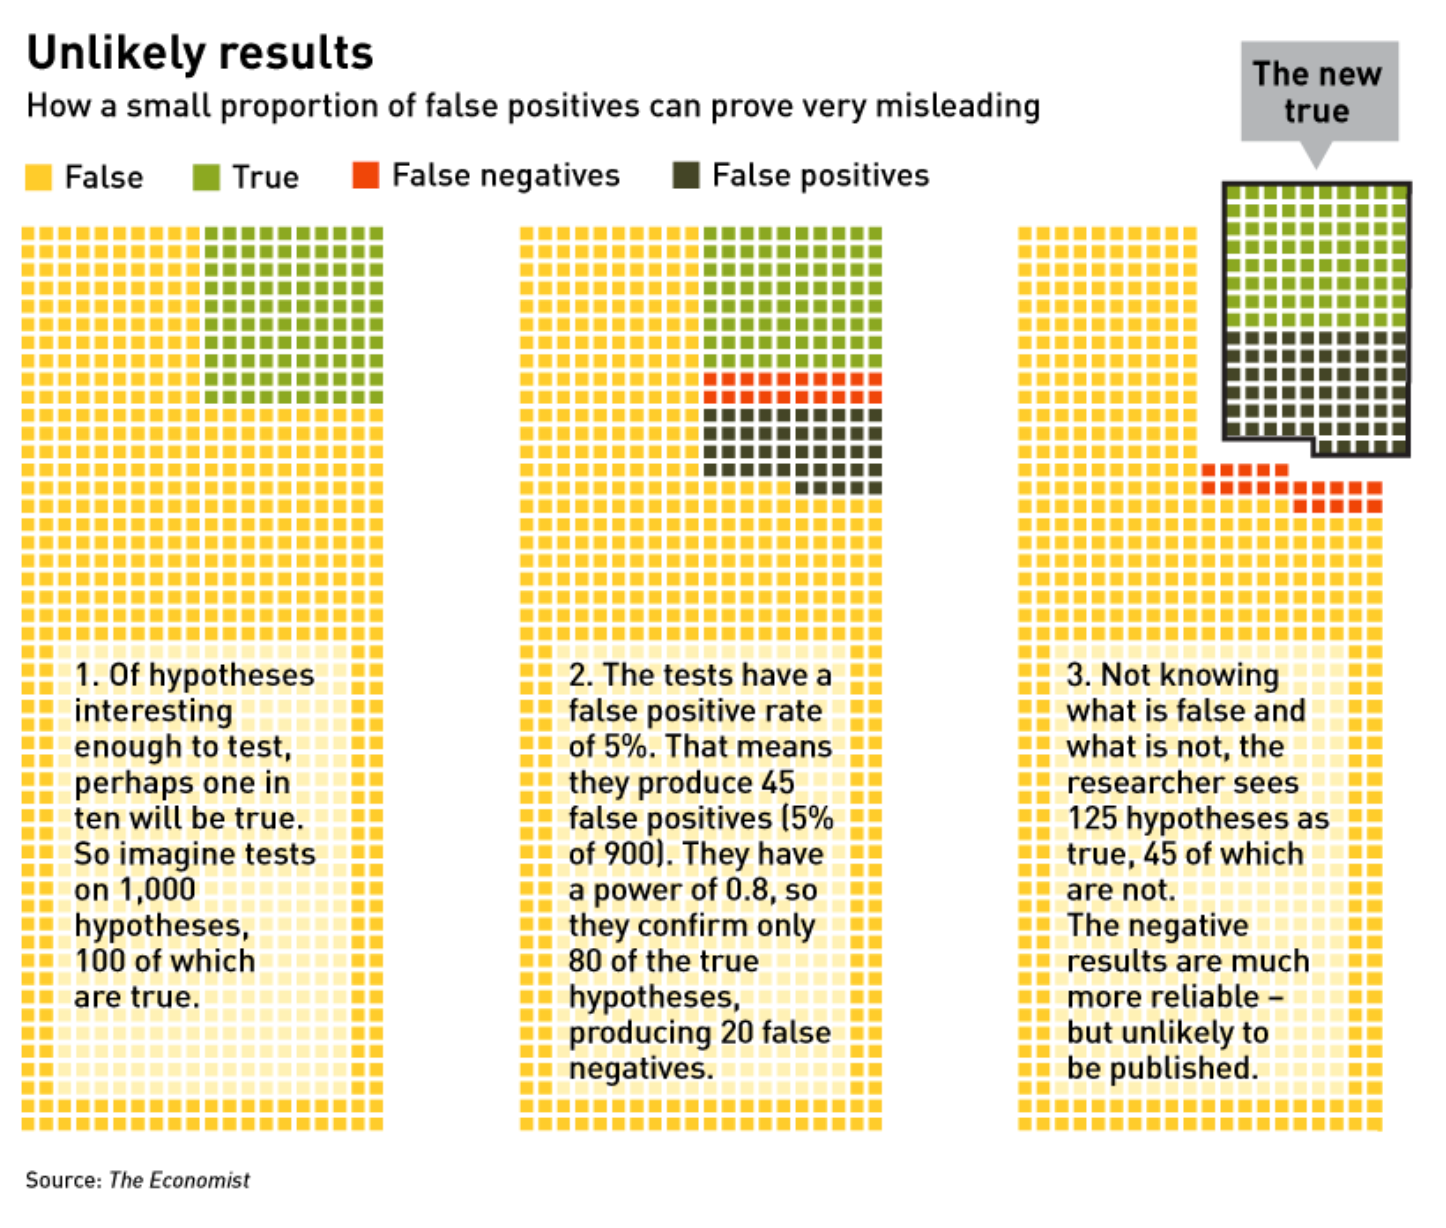
\includegraphics[width=0.9\linewidth]{figures/unlikely_results.png}
    \end{center}
\end{frame}


\begin{frame}
    \frametitle{Unlikely Results}
    
    \begin{center}
        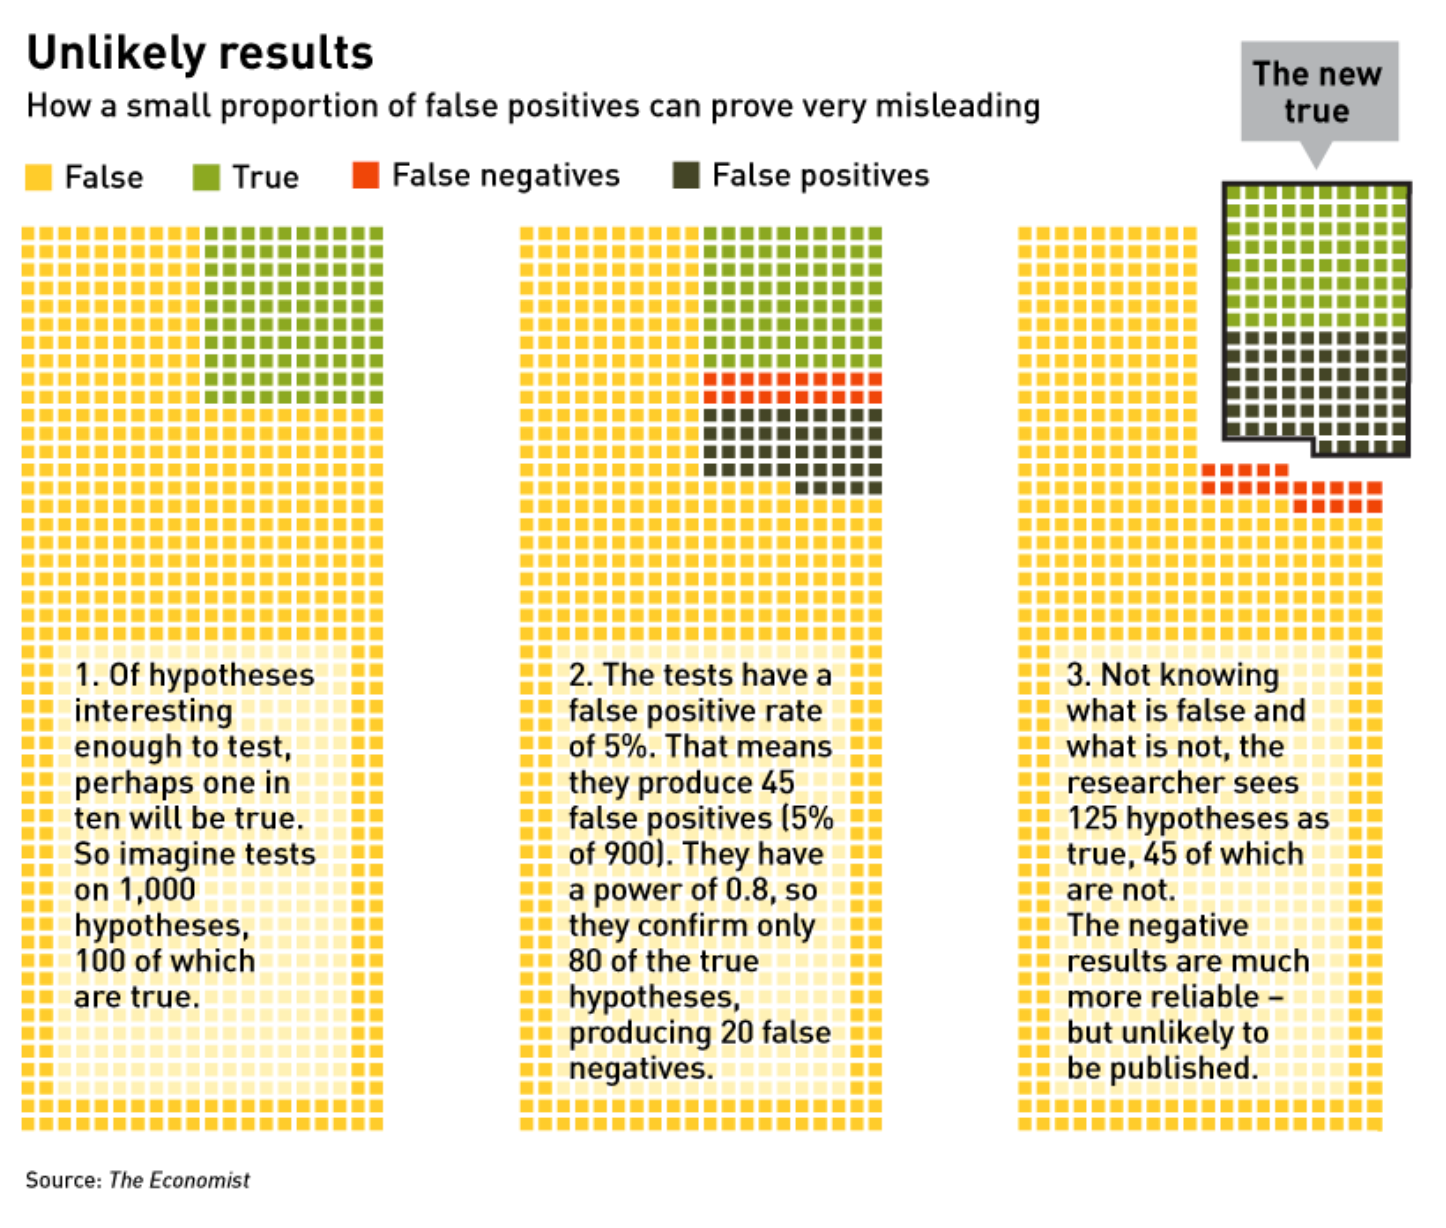
\includegraphics[width=0.75\linewidth]{figures/unlikely_results.png}
    \colorbox{burntOrange}
        {\textbf{PPV = 80/125 = 64\%} }

    \end{center}
\end{frame}


\begin{frame}
    \frametitle{Conclusion}
    
    \textbf{What is R? How many of the relationships we test are actually true?}
    \begin{itemize}
        \item It's hard to know, and it depends on the field you work in
        \item If you're testing different genes to see which ones can have a beneficial effect against some disease, the number of true relationships could be extremely small
        \item If you're working with socio-demographic variables, relationships are everywhere
        \begin{itemize}
            \item It's usually implausible to believe that two variables have exactly zero relationship
            \item Statistician Andrew Gelman claims he's never made a Type I error
            \item On the other hand, he does have to worry about a type S error: supporting a relationship but giving it the wrong sign
            \begin{itemize}
                \item Eg. claiming there's a positive relationship when the real relationship is negative
            \end{itemize}
            \item Think about the field that you work in and how this model might inform the way you interpret results
        \end{itemize}
    \end{itemize}
\end{frame}


\subsection{Solutions?}

\begin{frame}
    \frametitle{More Replication}
    
    {\large \textbf{Replication is still the final line of defense against errors: Can we find a way to encourage more of it?} }
    
    \vspace{0.1in}
    
    \textbf{Several authors have argued that we should start with students}
    \begin{itemize}
        \item Make replication a component of method classes
        \item A lot of students conduct class projects that don't have enough content for publication, but they might be harnessed to replicate established findings
        \item Students can also be trained on how to conduct meta-analysis
    \end{itemize}
    
    \vspace{0.1in}
    
    \textbf{Journals have a role to play, too}
        \begin{itemize}
            \item They can place a higher value on replication attempts
            \item Some journals are doing a good job (for example, the journal \textit{Social Psychology} recently devoted a special issue to replication studies
        \end{itemize}

\end{frame}
 
 
 \begin{frame}
     \frametitle{More Replication (cont.)}
     
    {\large \textbf{Replication is still the final line of defense against errors: Can we find a way to encourage more of it?} }
    
    \vspace{0.1in}
         
    \textbf{Authors can also make it easier to replicate their work}
    \begin{itemize}
        \item Publishing their data and their code
        \item A number of online repositories are trying to help with these issues
    \end{itemize}
    
    \vspace{0.1in}
        
    \textbf{In the end, the culture has to change}
    \begin{itemize}
        \item From students to the most famous researchers, everyone needs to value replication
        \item Psychology and medicine are now ahead of the game
        \item After suffering a major loss in confidence, these fields are really more willing to reform
    \end{itemize}

\end{frame}


\begin{frame}
    \frametitle{Pre-registration (Part 1)}
    
    \textbf{The idea is that researchers publish their research plans before gathering data}
    \begin{itemize}
        \item All methods of analysis in as much detail as possible
        \item All the tests that the researchers will run
    \end{itemize}
    
    \vspace{0.25in}
    
    \textbf{This helps in several ways}
    \begin{enumerate}
        \item It ties researchers' hands, 
        \begin{itemize}
            \item Fewer researcher degrees of freedom
            \item Less chance of Type I error inflation
        \end{itemize} 
        \item Ensures that we hear about studies, so negative results are less likely to fall into the file drawer
        \item Also encourages researchers to think clearly about proper research design ahead of time
    \end{enumerate}
\end{frame}


\begin{frame}
    \frametitle{Pre-registration (Part Two)}
    
    \textbf{Some journals in psychology and medicine are working to facilitate this with registered reports}
    \begin{itemize}
        \item Authors submit their research plans for peer review before collecting data
        \item Once properly reviewed, the authors get a provisional guarantee that their results will be published, whether negative or positive
        \item This reflects the fact that the best designs aren't necessarily the ones that lead to positive results; we should be able to judge them ahead of time.
    \end{itemize}
    
    \vspace{0.2in}
    
    \textbf{One problem is that it can be quite difficult to specify everything that you'll do in executing a study}
    \begin{itemize}
        \item There are just too many small decisions that have to go into an analysis
    \end{itemize}
\end{frame}


\begin{frame}
    \frametitle{Pre-registration (Part Three)}
    
    \textbf{It can help to begin with a small pilot study}
    \begin{itemize}
        \item This is a chance to write your code and refine your protocol
        \item Once this is done, you get your new data and plug it into your analysis script
        \item This is a great way to limit researcher degrees of freedom and make a study easier to replicate
    \end{itemize}
\end{frame}


\begin{frame}
    \frametitle{Fewer \textit{p-}Values}
    
    \textbf{\textit{p-}Values have taken a surprising amount of heat recently}
    \begin{itemize}
        \item A lot of researchers have spoken out, saying that we shouldn't be using \textit{p-}values at all or that we should de-emphasize them
        \item There's a general sense that \textit{p-}values are problematic
    \end{itemize}
    
    {\small \textit{"Second, in response to renewed recognition of the severe flaws of null-hypothesis significance testing (NHST), we need to shift from reliance on NHST to estimation and other preferred techniques. The new statistics refers to recommended practices, including estimation based on effect sizes, confidence intervals, and meta-analysis."}}
    \begin{flushright}
        -Geoff Cumming
    \end{flushright}     
    
    \textbf{A common argument is that a \textit{p-}value does not capture all the things that are important in interpreting a research result }
\end{frame}

\begin{frame}
    \frametitle{Fewer \textit{p-}Values (cont.)}

    \textbf{The cutoff at .05 is arbitrary}
    \begin{itemize}
        \item Relying on it causes publication bias and creates incentives for researchers to hack their \textit{p-}values
        \item It's possible that using confidence intervals will help shift the culture away from one that prioritizes positive results, and more toward one that focuses on replication and meta-analysis.
    \end{itemize}
    
    \textbf{At the same time, the problem isn't exactly \textit{p-}values; it's the lazy use of \textit{p-}values}
    \begin{itemize}
        \item \textit{p-}values are a summary measure
        \item They are a way that we can always describe the agreement between a statistic and a hypothesis
        \item There's danger other summary statistics will also be misapplied
        \item No matter what, researchers have to consider the wider research context and evaluate results critically
    \end{itemize}
    
    \textbf{I encourage you to form your own opinion on this debate}
    
\end{frame}


\begin{frame}
    \frametitle{The Nature of Research}
    
    \textbf{As you can see, there's no one solution that's going to solve the replication crisis}
    
    \vspace{0.2in}
    
    \begin{block}{Keep this in mind:}
        \textbf{Advancing scientific knowledge is hard}
    \end{block}
    
    \vspace{0.2in}
    
    \textbf{Our tools for gaining knowledge are imperfect}
    \begin{itemize}
        \item We have to work through human institutions
        \item We have limited resources
        \item There's a lot to learn to conduct research responsibly
    \end{itemize}
    
    \vspace{0.2in}
    
    \textbf{We have to be constantly vigilant and examine our methods}
    \begin{itemize}
        \item Be open to reform
    \end{itemize}
\end{frame}

\begin{frame}
    \frametitle{Conclusion}
    
    {\large 
        \textbf{I hope that this lecture has made you more aware of how the scientific method works}
        
        \vspace{0.25in}
    
        \textit{Whether in academia or industry, I hope that you will strive to be a responsible member of the research community and help us move toward a more effective use of statistics}
    }
\end{frame}


\end{document}
